\documentclass[10pt]{beamer}

\usetheme[progressbar=foot, background=dark]{metropolis}
\usepackage{appendixnumberbeamer}

% fsts
\usepackage{tikz}
% strikethrough
\usepackage[normalem]{ulem}
% code listing thing
\usepackage{listings}

\usepackage{color}

\definecolor{codegreen}{rgb}{0,0.6,0}
\definecolor{codegray}{rgb}{0.5,0.5,0.5}
\definecolor{codepurple}{rgb}{0.58,0,0.82}
\definecolor{backcolour}{rgb}{0.95,0.95,0.92}

\lstdefinestyle{mystyle}{
    commentstyle=\color{codegreen},
    keywordstyle=\color{magenta},
    numberstyle=\tiny\color{codegray},
    stringstyle=\color{codepurple},
    basicstyle=\tiny,
    breakatwhitespace=false,
    breaklines=true,
    captionpos=b,
    keepspaces=false,
    numbers=left,
    numbersep=5pt,
    showspaces=false,
    showstringspaces=false,
    showtabs=false,
    tabsize=2
}

\lstset{style=mystyle}

\usepackage{booktabs}
\usepackage[scale=2]{ccicons}

\usepackage{pgfplots}
\usepgfplotslibrary{dateplot}

\usepackage{subfigure}
\usepackage{gb4e}

\usepackage{xspace}
\newcommand{\themename}{\textbf{\textsc{metropolis}}\xspace}
\graphicspath{{figs/}}

\title{Things* I wish I knew* before starting an industry job}
\subtitle{TODO:explain *}
\date{February 23, 2018}
\author{Trevor Sullivan}
% \institute{University of Arizona}
% \titlegraphic{\hfill\includegraphics[height=1.5cm]{logo.pdf}}

\begin{document}

\maketitle

\begin{frame}{Background in 30 seconds, GO!}
\pause
    \begin{itemize}[<+->]
    	\item Came to UofAZ as a music/linguistics student
    	\item Realized music is a dumb thing to spend \$40,000 on
    	\item Hey computers are cool
    	\item Double major in linguistics/CS
    	\item Masters program? hell yeah!
    	\item Internship with ayfie on fuzzy prefix search
    	\item Job?
    	\item yes
    	\item search for lawyers
    \end{itemize}
\pause
TIME

\end{frame}

\begin{frame}{Overview}
\pause
\begin{itemize}[<+->]
	\item I worked as an intern for ayfie for my hlt project on fuzzy prefix search
	(cf October 2016 Data Science Meetup)
	\item I was hired afterwards as a Professional Service Engineer, to start in May
	\item I took some notes on things* that I found particularly frustrating to not know* ahead of time
\end{itemize}
\pause
Starting any new job comes with a learning phase that lasts weeks or months, but knowing* about some things* ahead of time will help you make the transition more easily

\end{frame}

\begin{frame}
	\frametitle{On things and knowing}

	\begin{itemize}[<+->]
		\item Things
		\begin{itemize}[<+->]
			\item This is just an excuse for me to bring up \alert{impostor syndrome} because it didn't fit anywhere else in the talk
			\item it never goes away
			\item \textbf{NOW} is the time to practice your confidence and self esteem
		\end{itemize}
		\item Knowing
		\begin{itemize}[<+->]
			\item knowing \textit{about}
			\item \textit{knowing} knowing
		\end{itemize}
	\end{itemize}
\end{frame}


\begin{frame}{Table of contents}
  \setbeamertemplate{section in toc}[sections numbered]
  \tableofcontents[hideallsubsections]
\end{frame}




















\section{Cluster computing | Functional programming}

\begin{frame}[c]\frametitle{Be aware of: Cluster computing}

Spark/Hadoop

\pause

\centerline{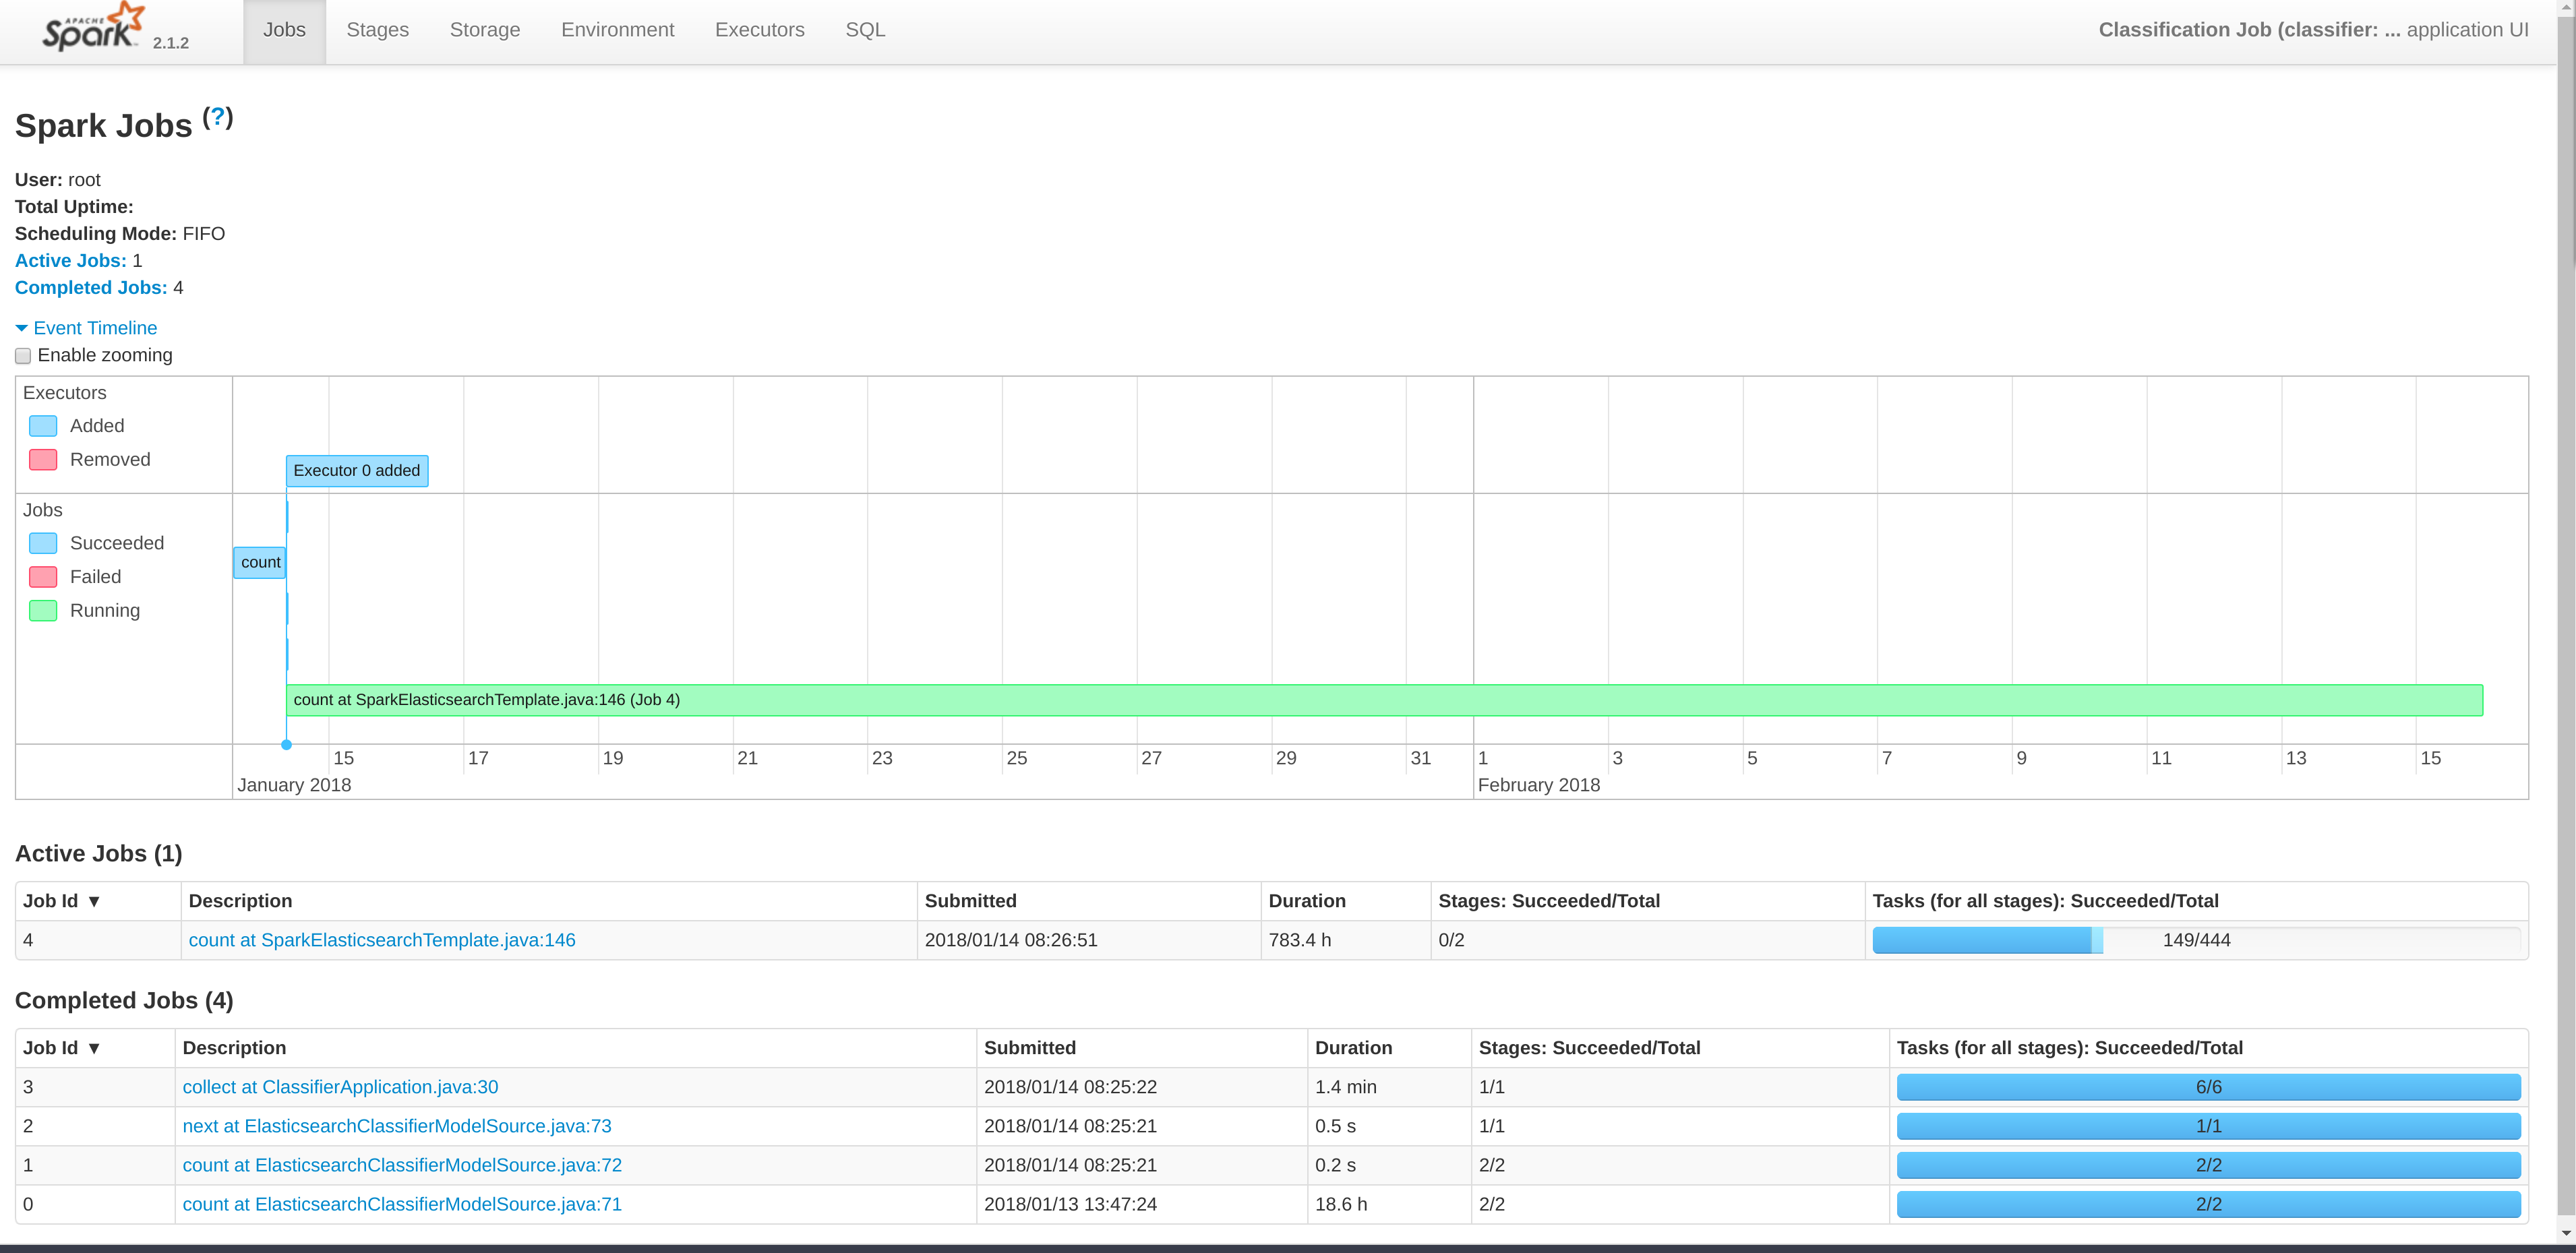
\includegraphics[width=10cm]{figs/spark.png}}

A way to distribute data and computation to make your stuff scalable.

Abstracts away parallelism and data structure so you can focus on functionality

\end{frame}


\begin{frame}[fragile]\frametitle{Do it now: Functional programming}

Cluster computing relies on functional programming, so you should definitiely be familiar with it.

These two code samples do the same thing.

\begin{columns}[T]
  \begin{column}{.48\textwidth}
  % \centerline{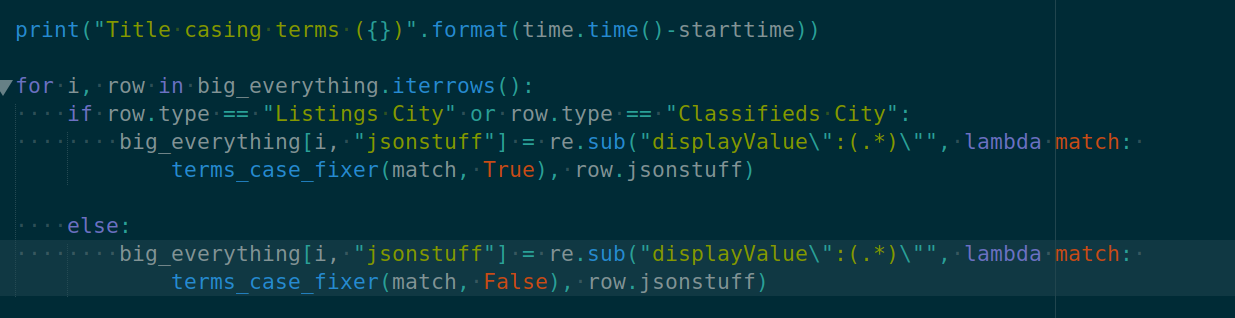
\includegraphics[width=6cm]{figs/slowpandasloop.png}}
  \begin{lstlisting}[language=Python]
for i, row in big_everything.iterrows():
  if row.type == "Listings City":
    big_everything[i,'jsonstuff'] = re.sub("displayValue\":(.*)\"", lambda m: case_fixer(m, True), row.jsonstuff)

  else:
    big_everything[i,'jsonstuff'] = re.sub("displayValue\":(.*)\"", lambda m: case_fixer(m, False), row.jsonstuff)

  \end{lstlisting}
  \pause
  10 hours
  \end{column}

  \pause


  \begin{column}{.48\textwidth}
  % \centerline{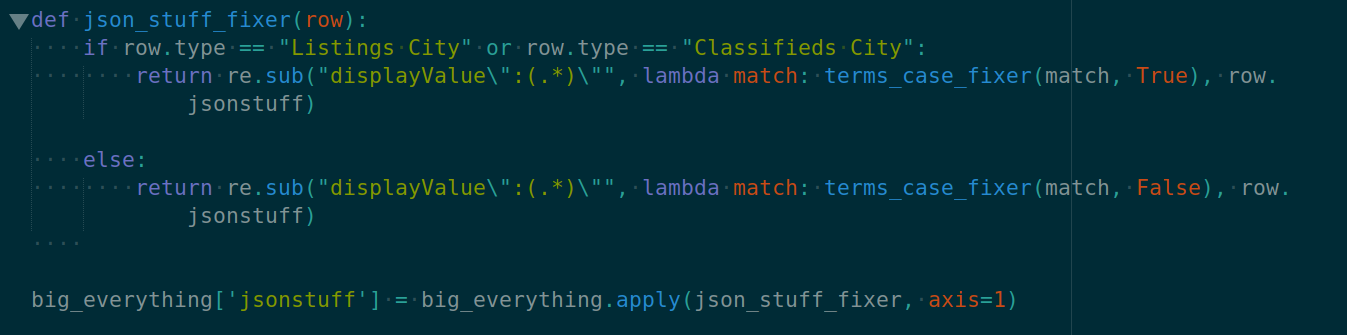
\includegraphics[width=6cm]{figs/fastpandasfunc.png}}
  % \centerline{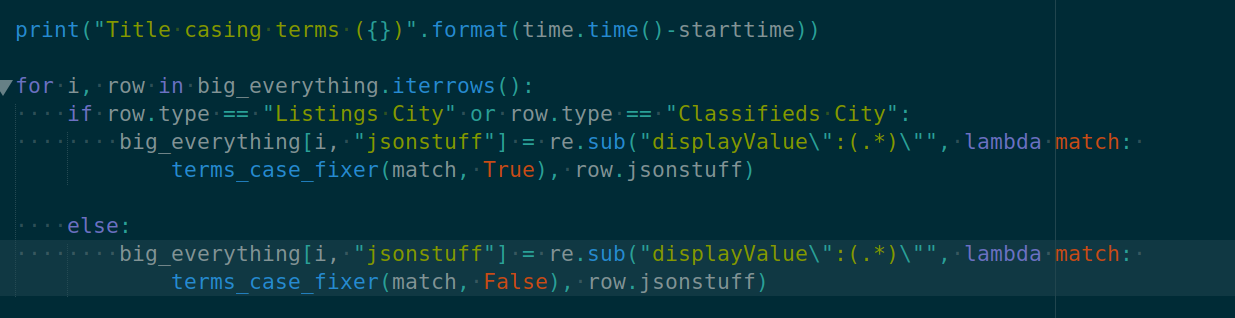
\includegraphics[width=6cm]{figs/slowpandasloop.png}}
  \begin{lstlisting}[language=Python]
def json_stuff_fixer(row):
  if row.type == "Listings City":
    return re.sub("displayValue\":(.*)\"", lambda m: case_fixer(m, True), row.jsonstuff)

  else:
    return re.sub("displayValue\":(.*)\"", lambda m: case_fixer(m, False), row.jsonstuff)


big_everything['jsonstuff'] = big_everything.apply(json_stuff_fixer, axis=1)
  \end{lstlisting}
  \pause


  4 minutes
  \end{column}
  \end{columns}

\end{frame}

\begin{frame}[c]\frametitle{Functional Programming}

    People who write functional/distributed database libraries are smarter than you.

    \pause

    If a functional idiom is available, \alert{use it}.

    \pause

    It requires you to think a different way from the typical OOP paradigm, but there is great benefit and a good mental exercise besides.

    Most important things to learn:
    \begin{itemize}
    	\item lambda
    	\item foreach
    	\item apply
    	\item map
    	\item filter
    	\item reduce
    \end{itemize}
\end{frame}





















\section{Continuous Integration | Testing}

\begin{frame}[c]\frametitle{Be aware of: Continuous Integration}

CI is a way of making sure that code you commit or push works.

\pause

In commercial applications, you will probably use Jenkins

\pause

\centerline{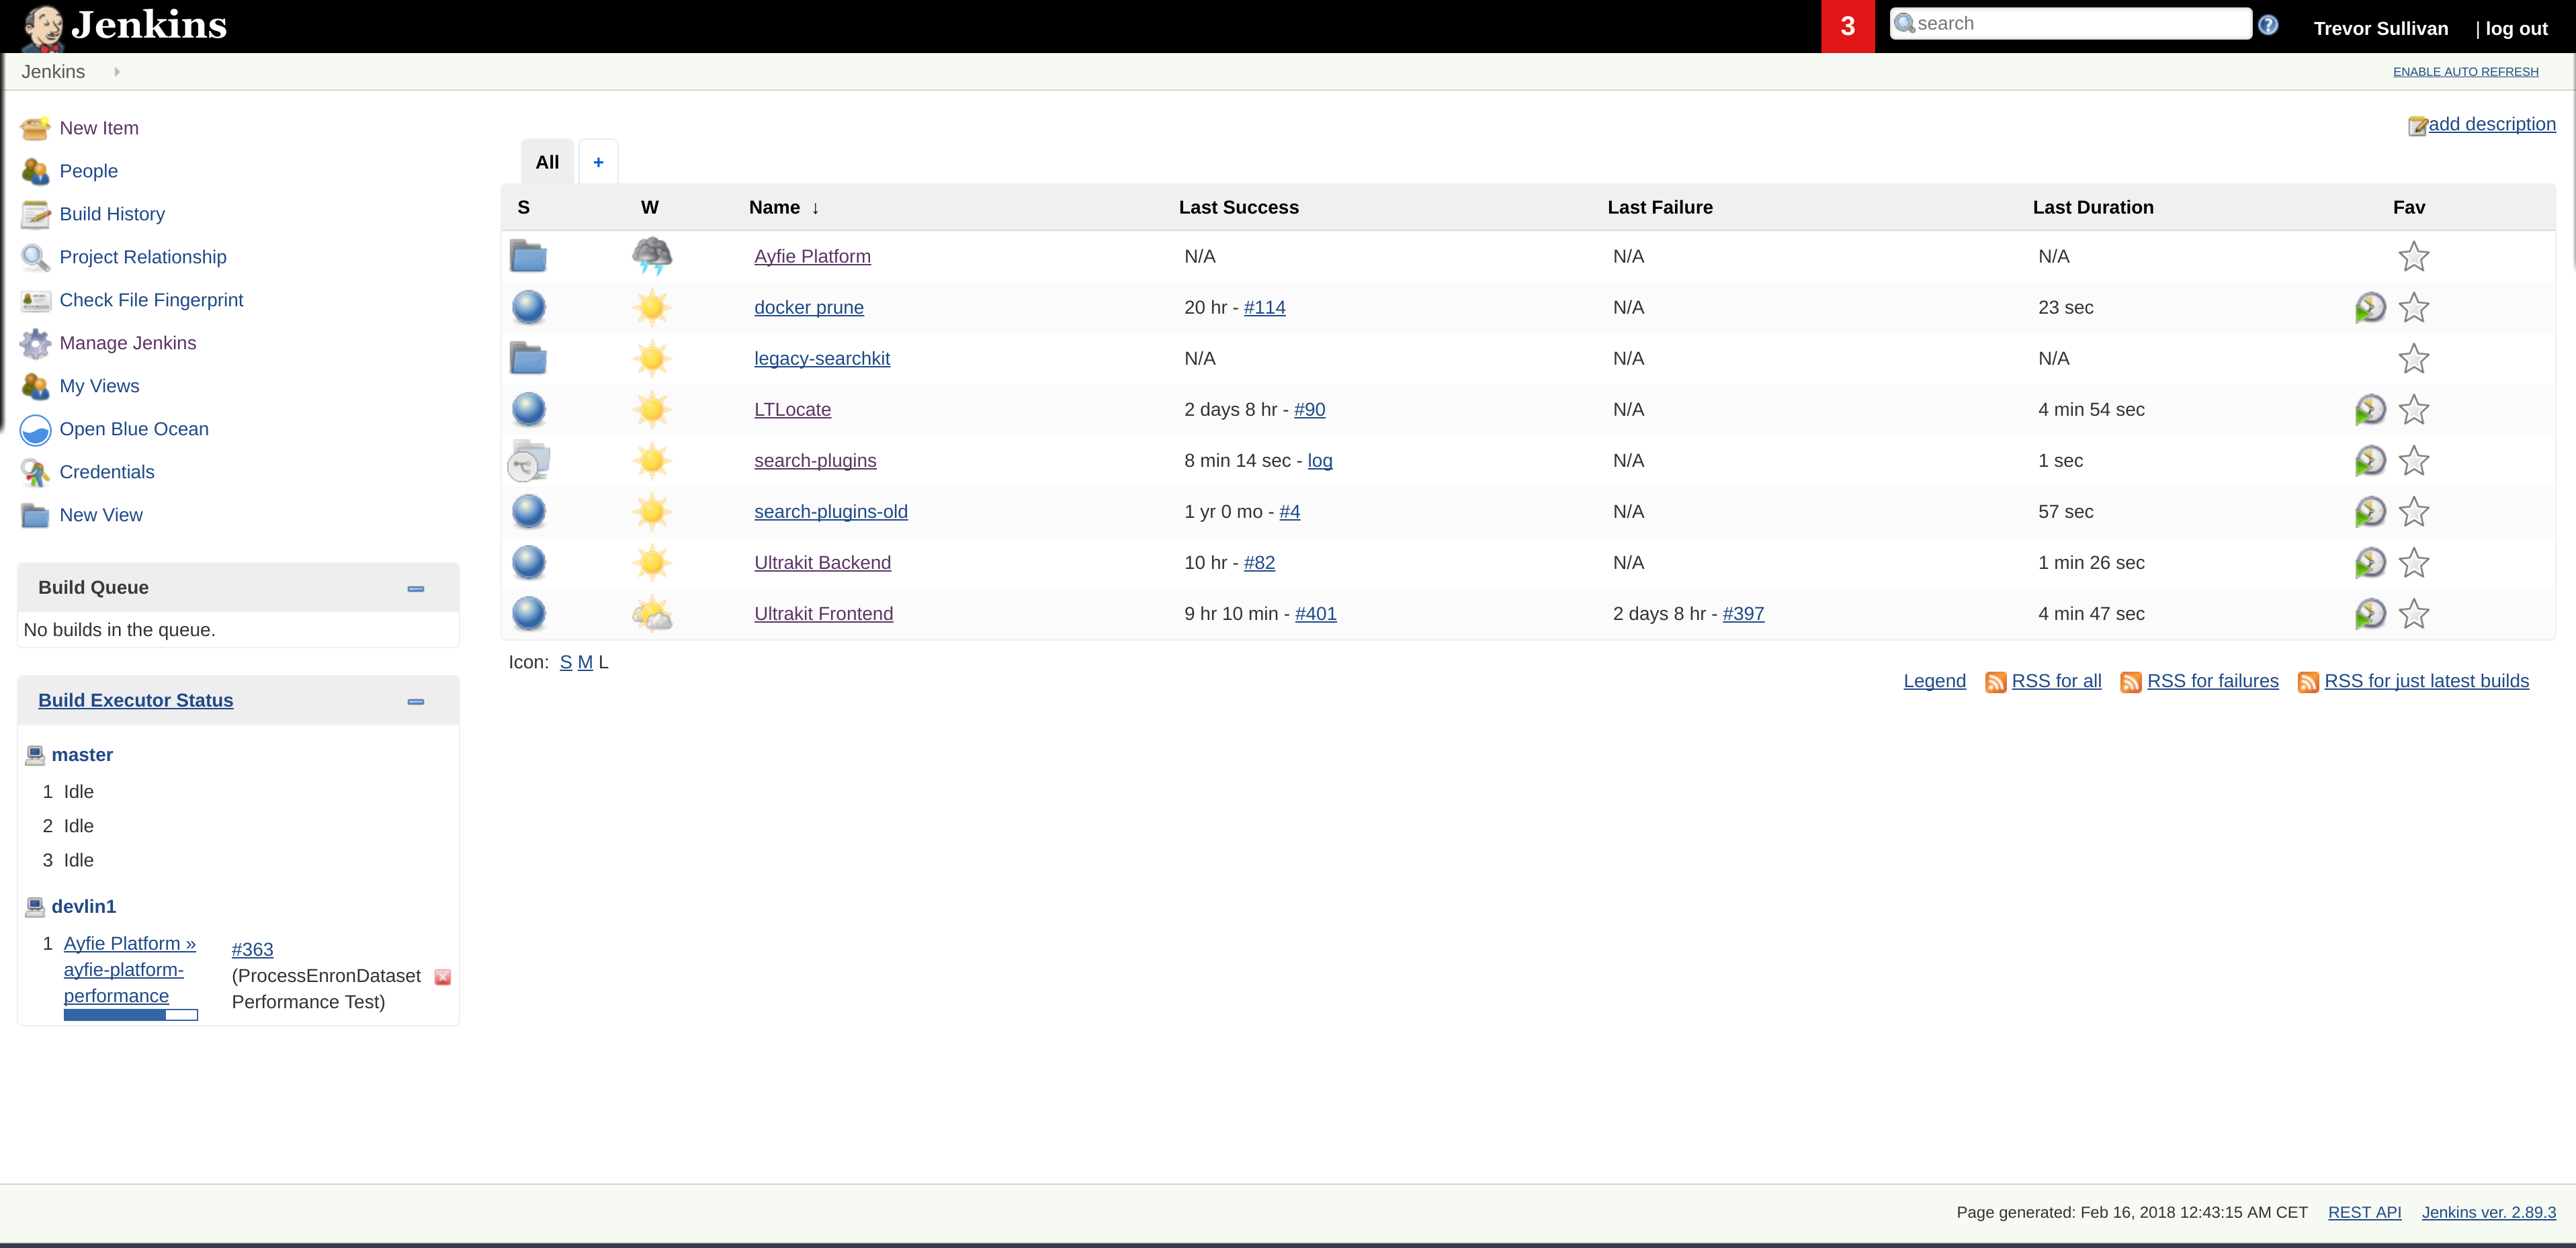
\includegraphics[width=10cm]{figs/jenkins.png}}

\pause

CI builds your code in a consistent environment and tests it to make sure it works.

\end{frame}


\begin{frame}[c]\frametitle{Travis}

\centerline{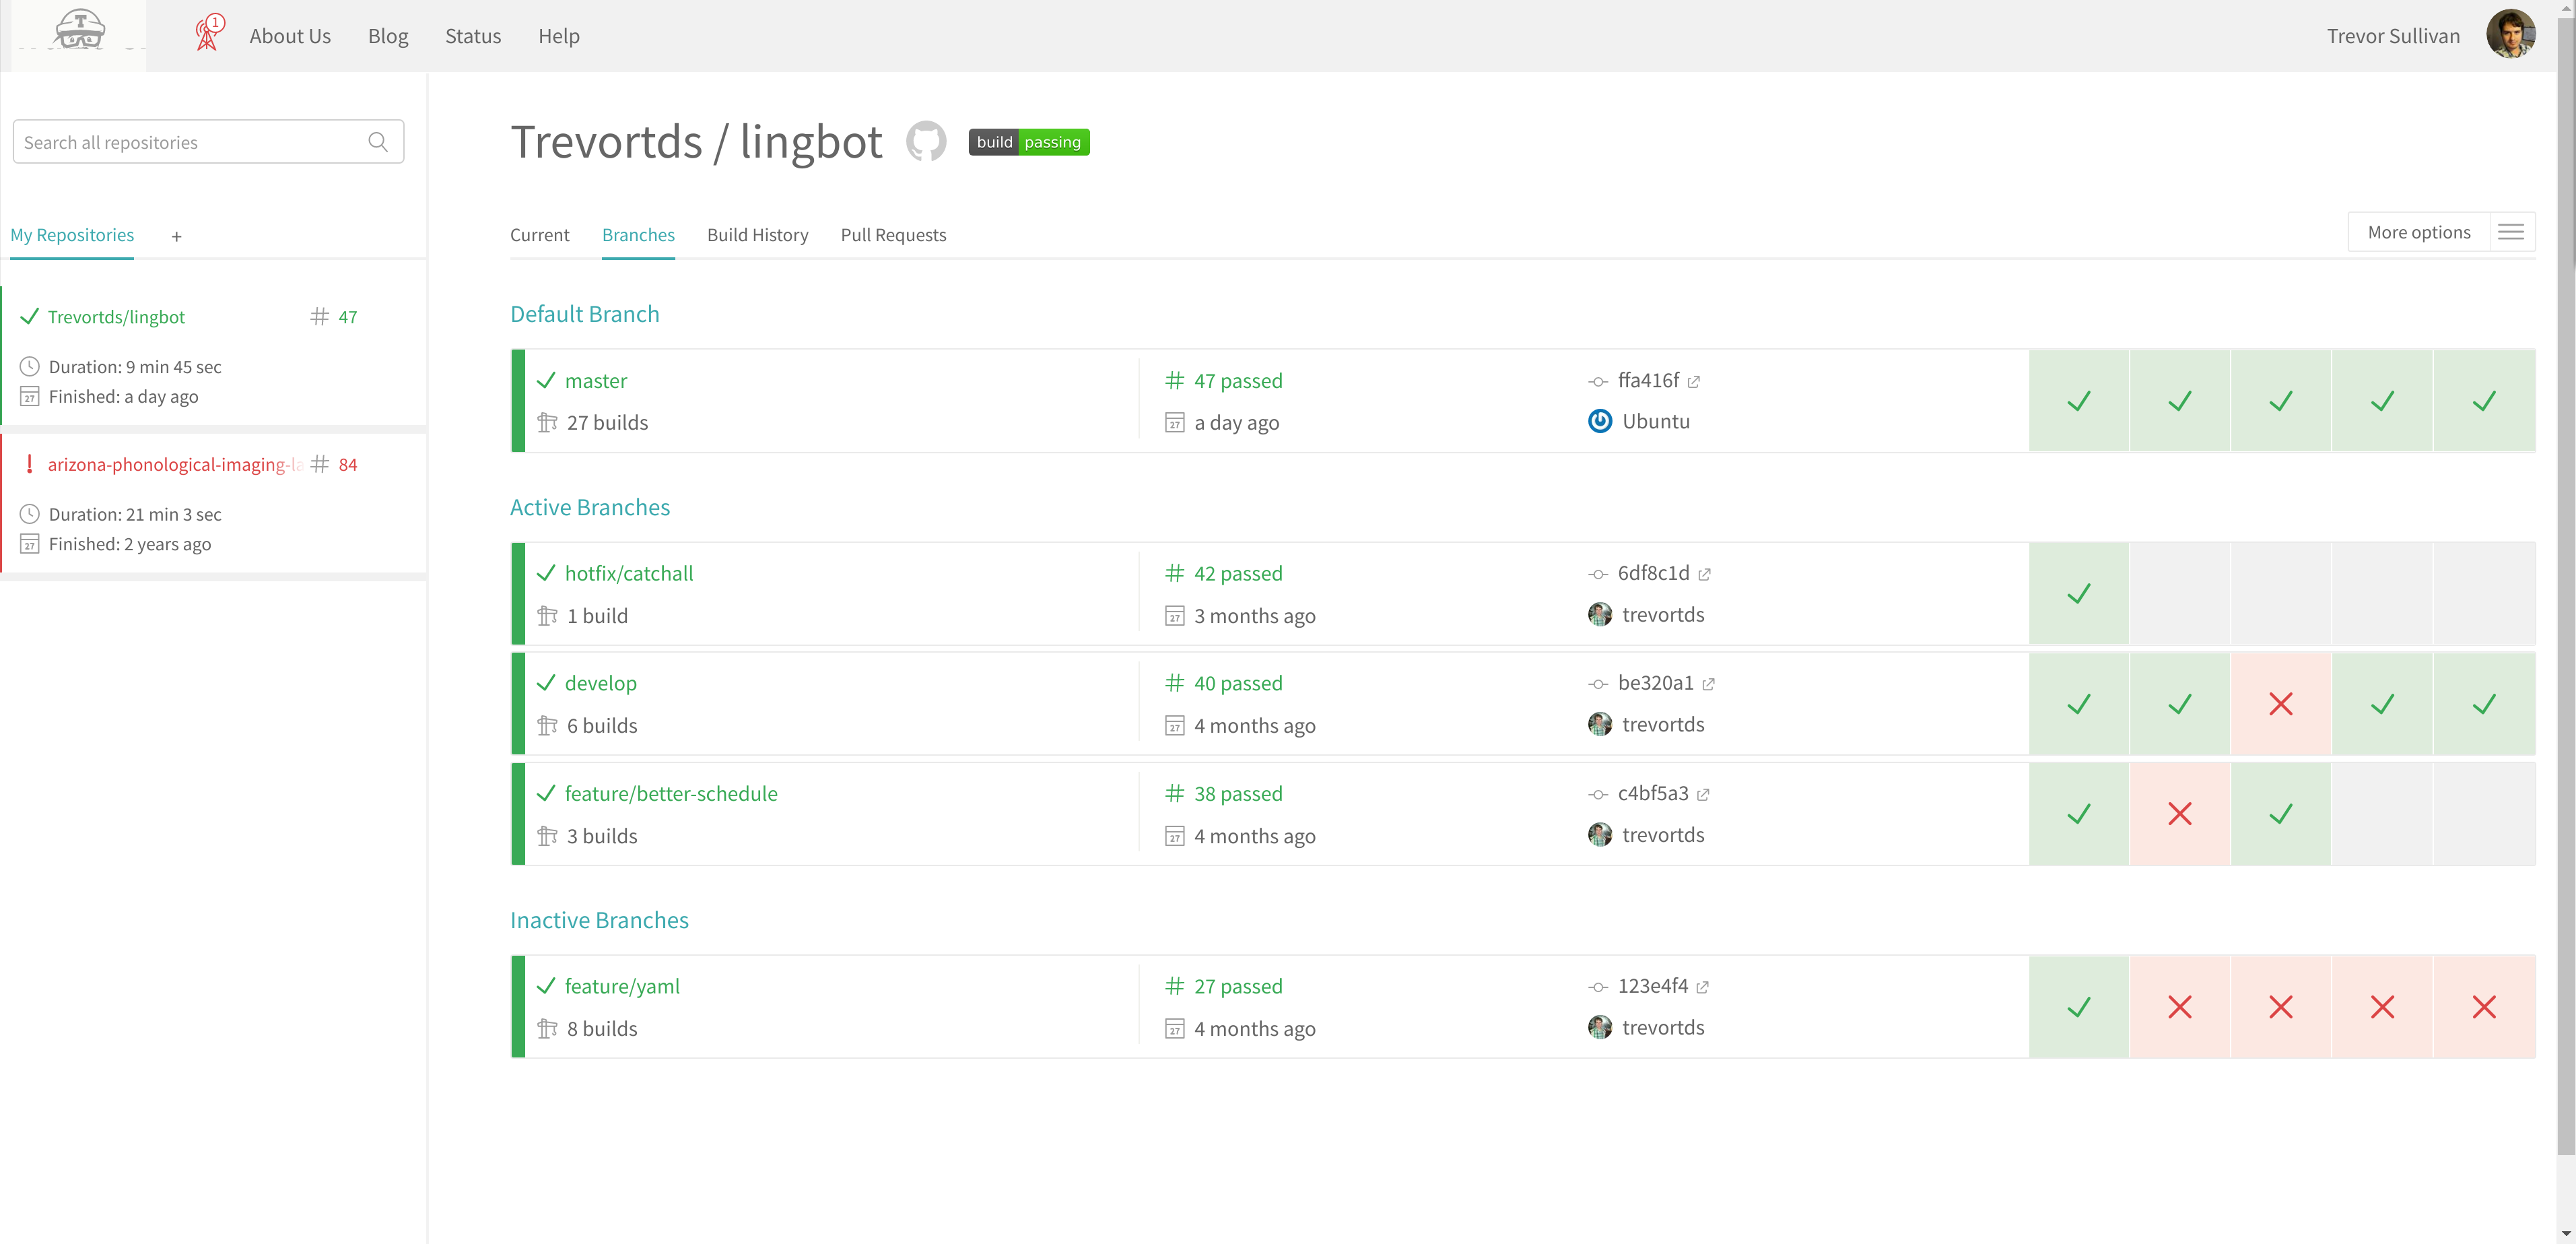
\includegraphics[width=11cm]{figs/travis.png}}

\end{frame}



\begin{frame}[c]\frametitle{Do it now: Testing}

\pause

OMG testing is great.

\pause

For medium-to-large size projects

\begin{enumerate}[<+->]
	\item Find bugs faster
	\item Find their causes faster
	\item Prevent problems from reoccurring
\end{enumerate}

\pause
There are testing systems out there for every language.

\begin{description}
	\item[Python] pytest
	\item[Java] junit
	\item[scala] scalatest
\end{description}

And you can set up your environment to run tests on every commit.

\end{frame}

\begin{frame}[c]\frametitle{How to write tests}
    There are three kinds of tests.

    \begin{description}[<+->]
    	\item[Unit tests] Test a method or function
    	\item[Regression tests] Duplicate known bugs
    	\item[Integration tests] Test interactions between modules
    \end{description}


\end{frame}

\begin{frame}[c]\frametitle{Unit test example}

    \centerline{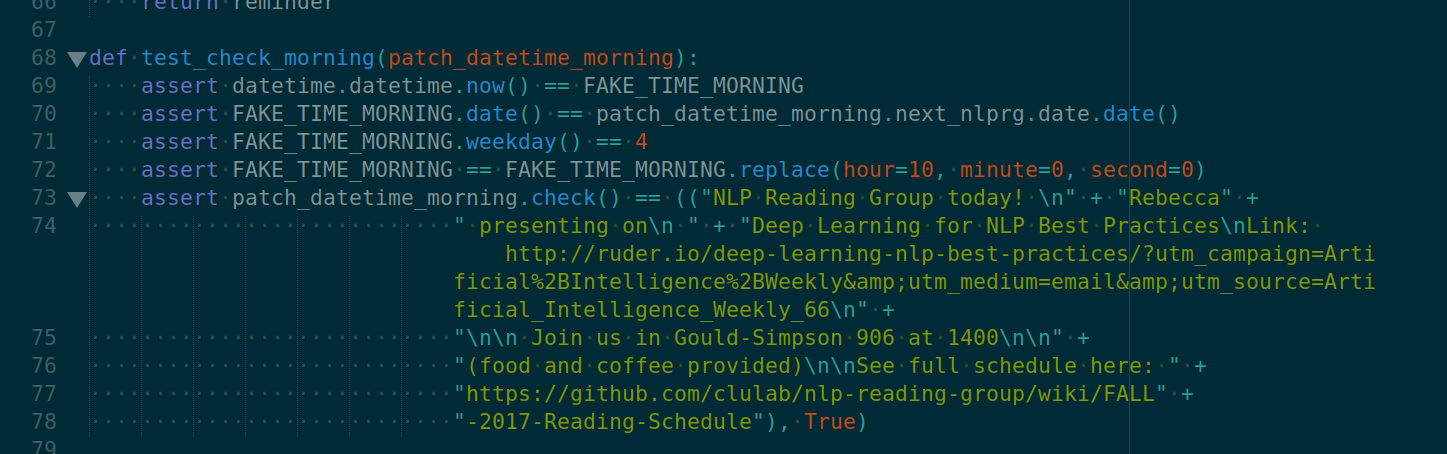
\includegraphics[width=10cm]{figs/lingbottest.png}}

    \pause

    Each unit test should look at one method and exemplify one edge case.

    \pause

    Forces you to think about how things could go wrong, and reveals them before they do.

\end{frame}



















\section{Docker, containerization, packaging | Git/Git-flow}

\begin{frame}[c]\frametitle{Be aware of: Docker, containerization, packaging}

\pause

Docker is a system for dedicated containers, mini VMs, that run just one application accessed over the network.

Docker lets you manage

\begin{itemize}[<+->]
	\item environment variables
	\item software versions
	\item port
	\item data locations
	\item including what to store and what to keep ephemeral
	\item custom binaries to inject
	\item memory and cpu limits
	\item system integration
	\item all kinds of cool stuff
\end{itemize}

\end{frame}

\begin{frame}[c]\frametitle{Using Docker}

Settings go into a docker-compose.yml

\centerline{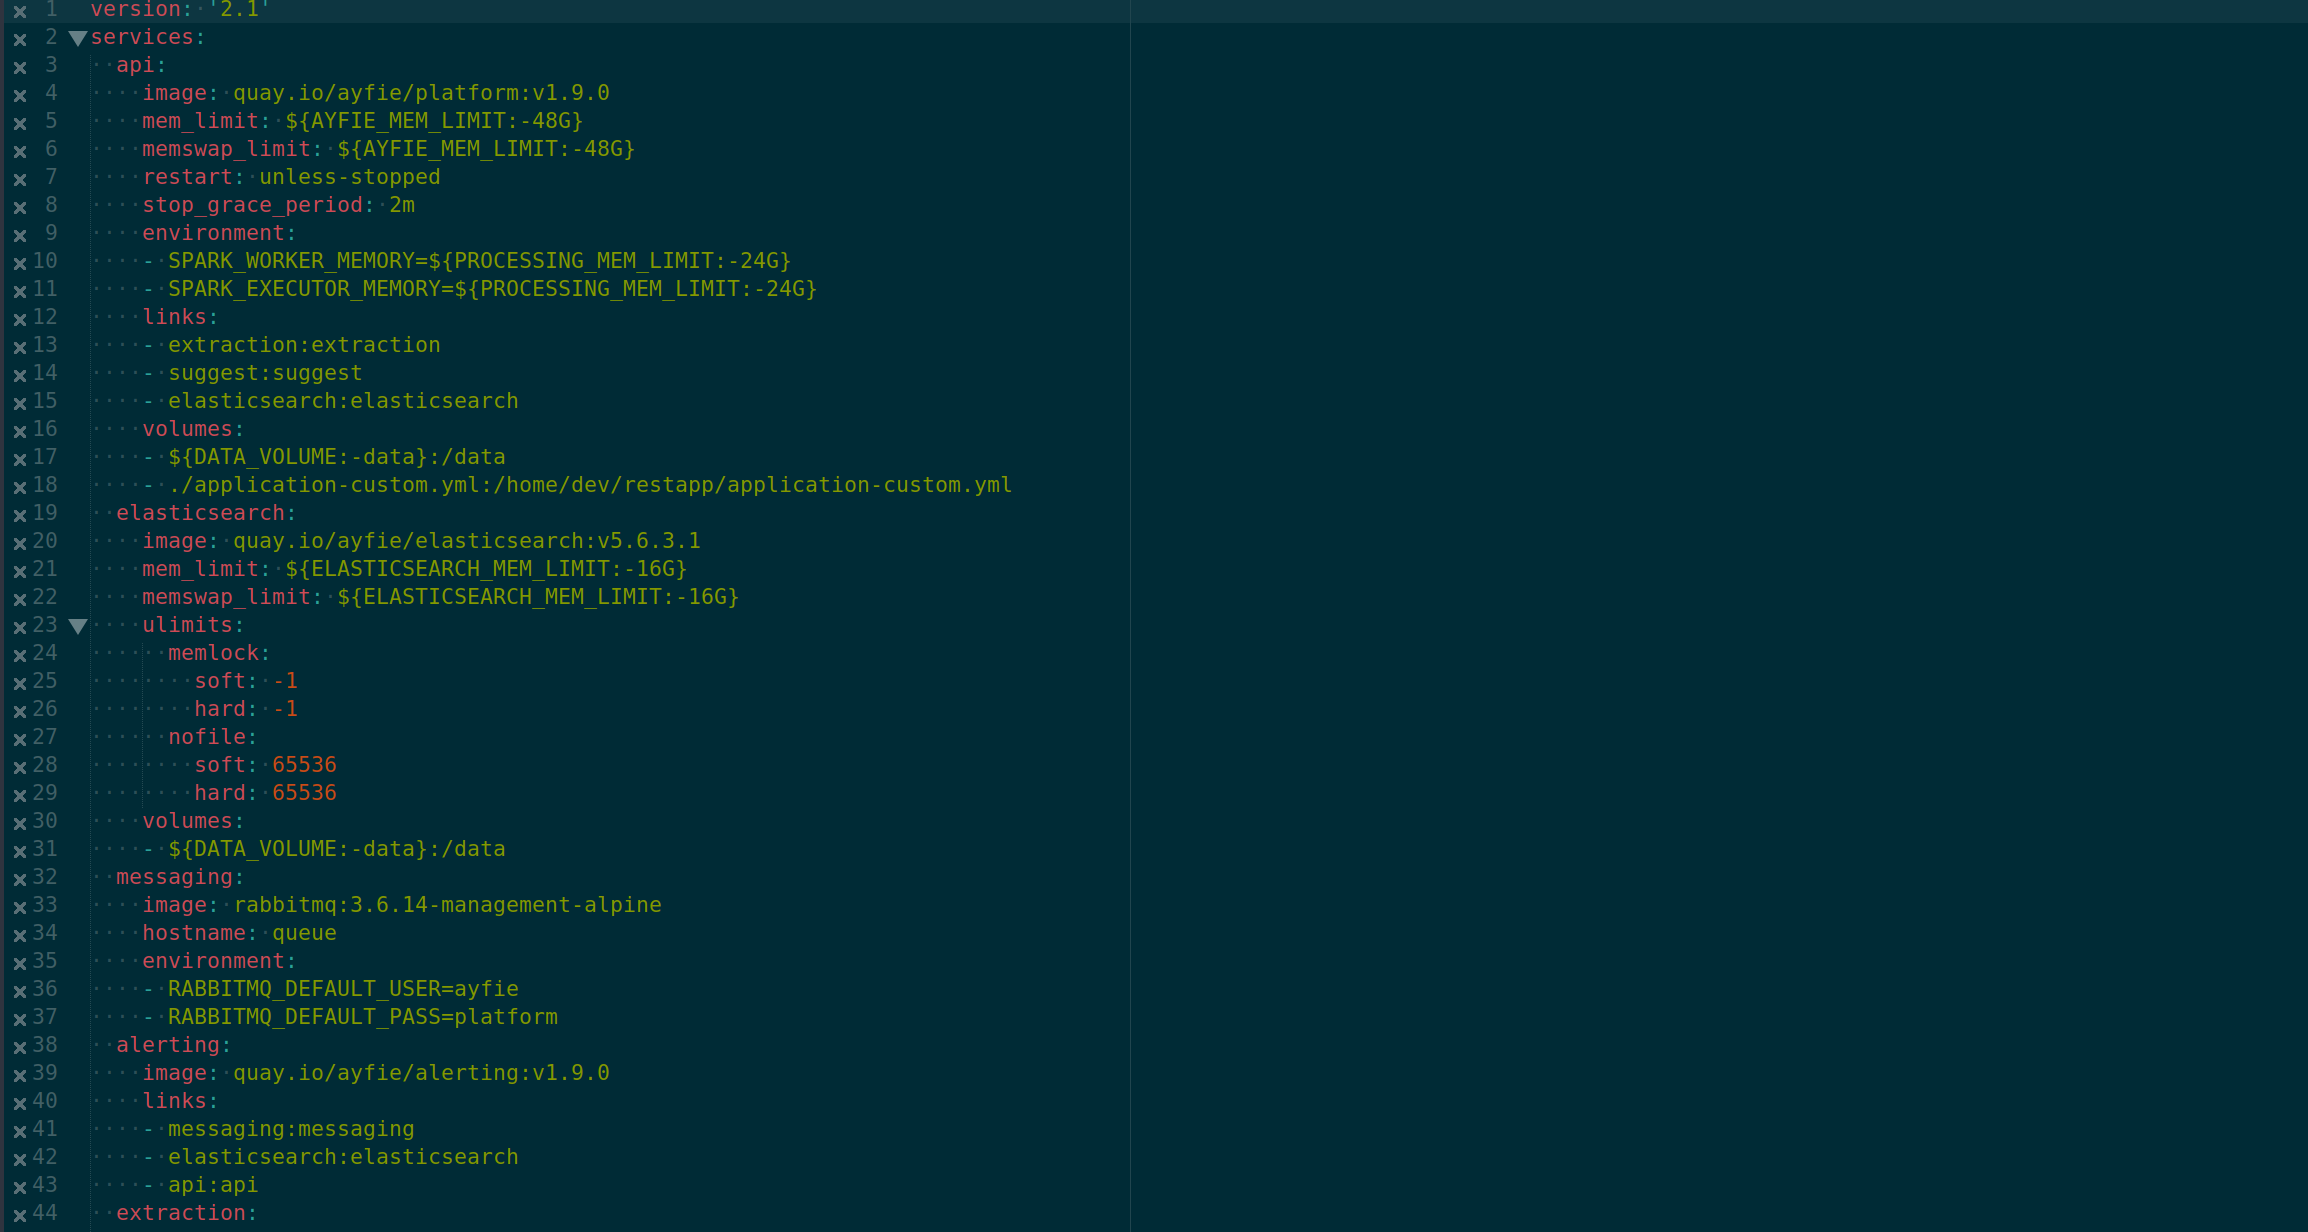
\includegraphics[width=10cm]{figs/dockercompose.png}}

And starting the system as a background service is as easy as \texttt{docker-compose up}


\end{frame}

\begin{frame}[c]\frametitle{Maybe consider: yaml for configuration}

Way easier than putting stuff at the top of each file, and more understandable than environment variables

\begin{columns}[T]
  \begin{column}{.48\textwidth}
  \centerline{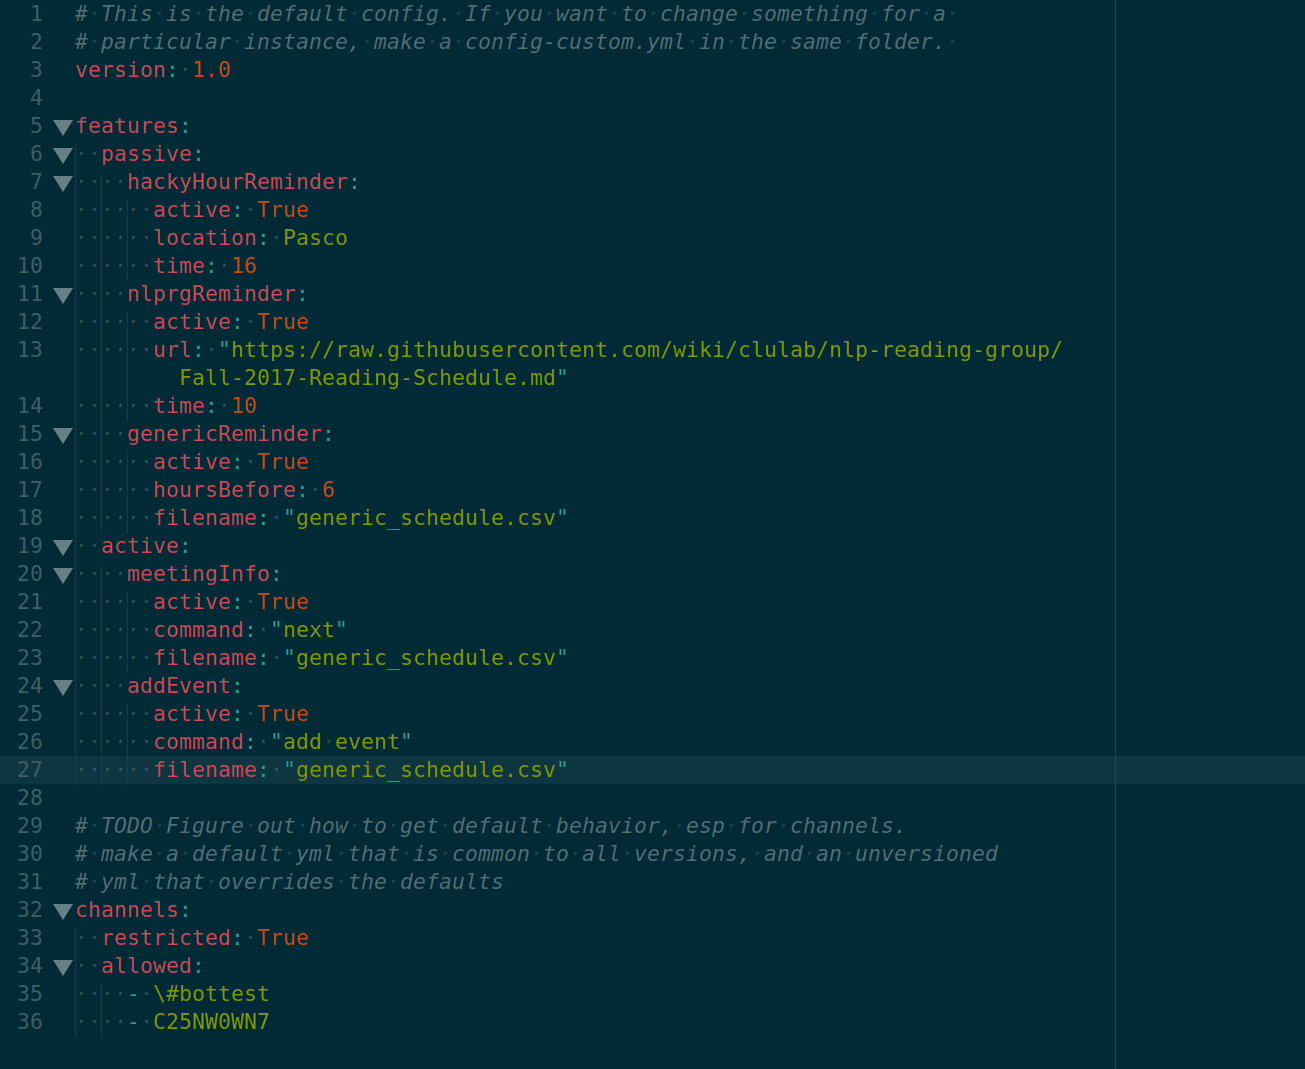
\includegraphics[width=6cm]{figs/lingbotyml.png}}
  \end{column}

  \pause



  \begin{column}{.48\textwidth}
  \centerline{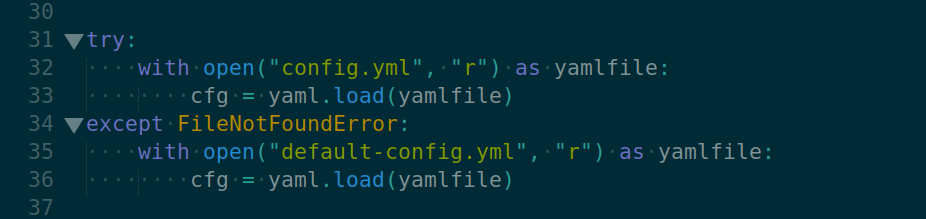
\includegraphics[width=6cm]{figs/lingbotymlsource.png}}


  \end{column}
  \end{columns}
\end{frame}


\begin{frame}[c]\frametitle{Do it now: Git everything!}

\begin{itemize}[<+->]
	\item We are all introduced to git for collaboration

	\pause

	\alert{\textbf{THAT'S NOT WHAT IT'S FOR}}

	\item Version Control

	\item Even if you don't have a repository

	\item Github, Gitlab, Bitbucket are nice for publishing and sharing, but you should be using git even if you don't want to share.

	\item \texttt{cd thing\_im\_working\_on ; git init}

\end{itemize}

\end{frame}

\begin{frame}[c]\frametitle{Do it now: Git Flow}
    For semester projects, theses, things you expect to be working on more than a week

    \pause

    \texttt{git flow init}

    \pause

    \centerline{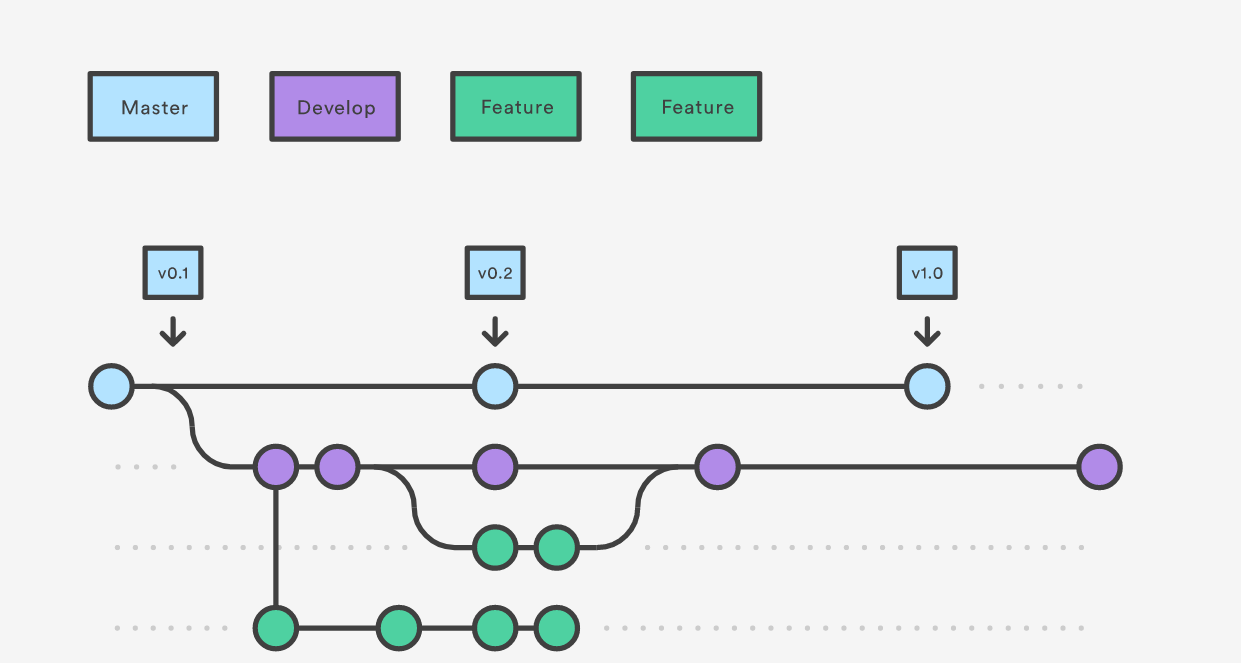
\includegraphics[width=11cm]{figs/gitflow.png}}


\end{frame}






\begin{frame}[standout]
  Check time!
\end{frame}




\appendix







\section{Team workflows | Personal task management}

\begin{frame}[c]
	\frametitle{Be aware of: Scrum and Team Workflows}
	\begin{itemize}[<+->]
		\item Every company does this a different way
		\item scrum master
		\item sprint review
		\item board
	\end{itemize}
\end{frame}

\begin{frame}[c]{Boards}
    \centerline{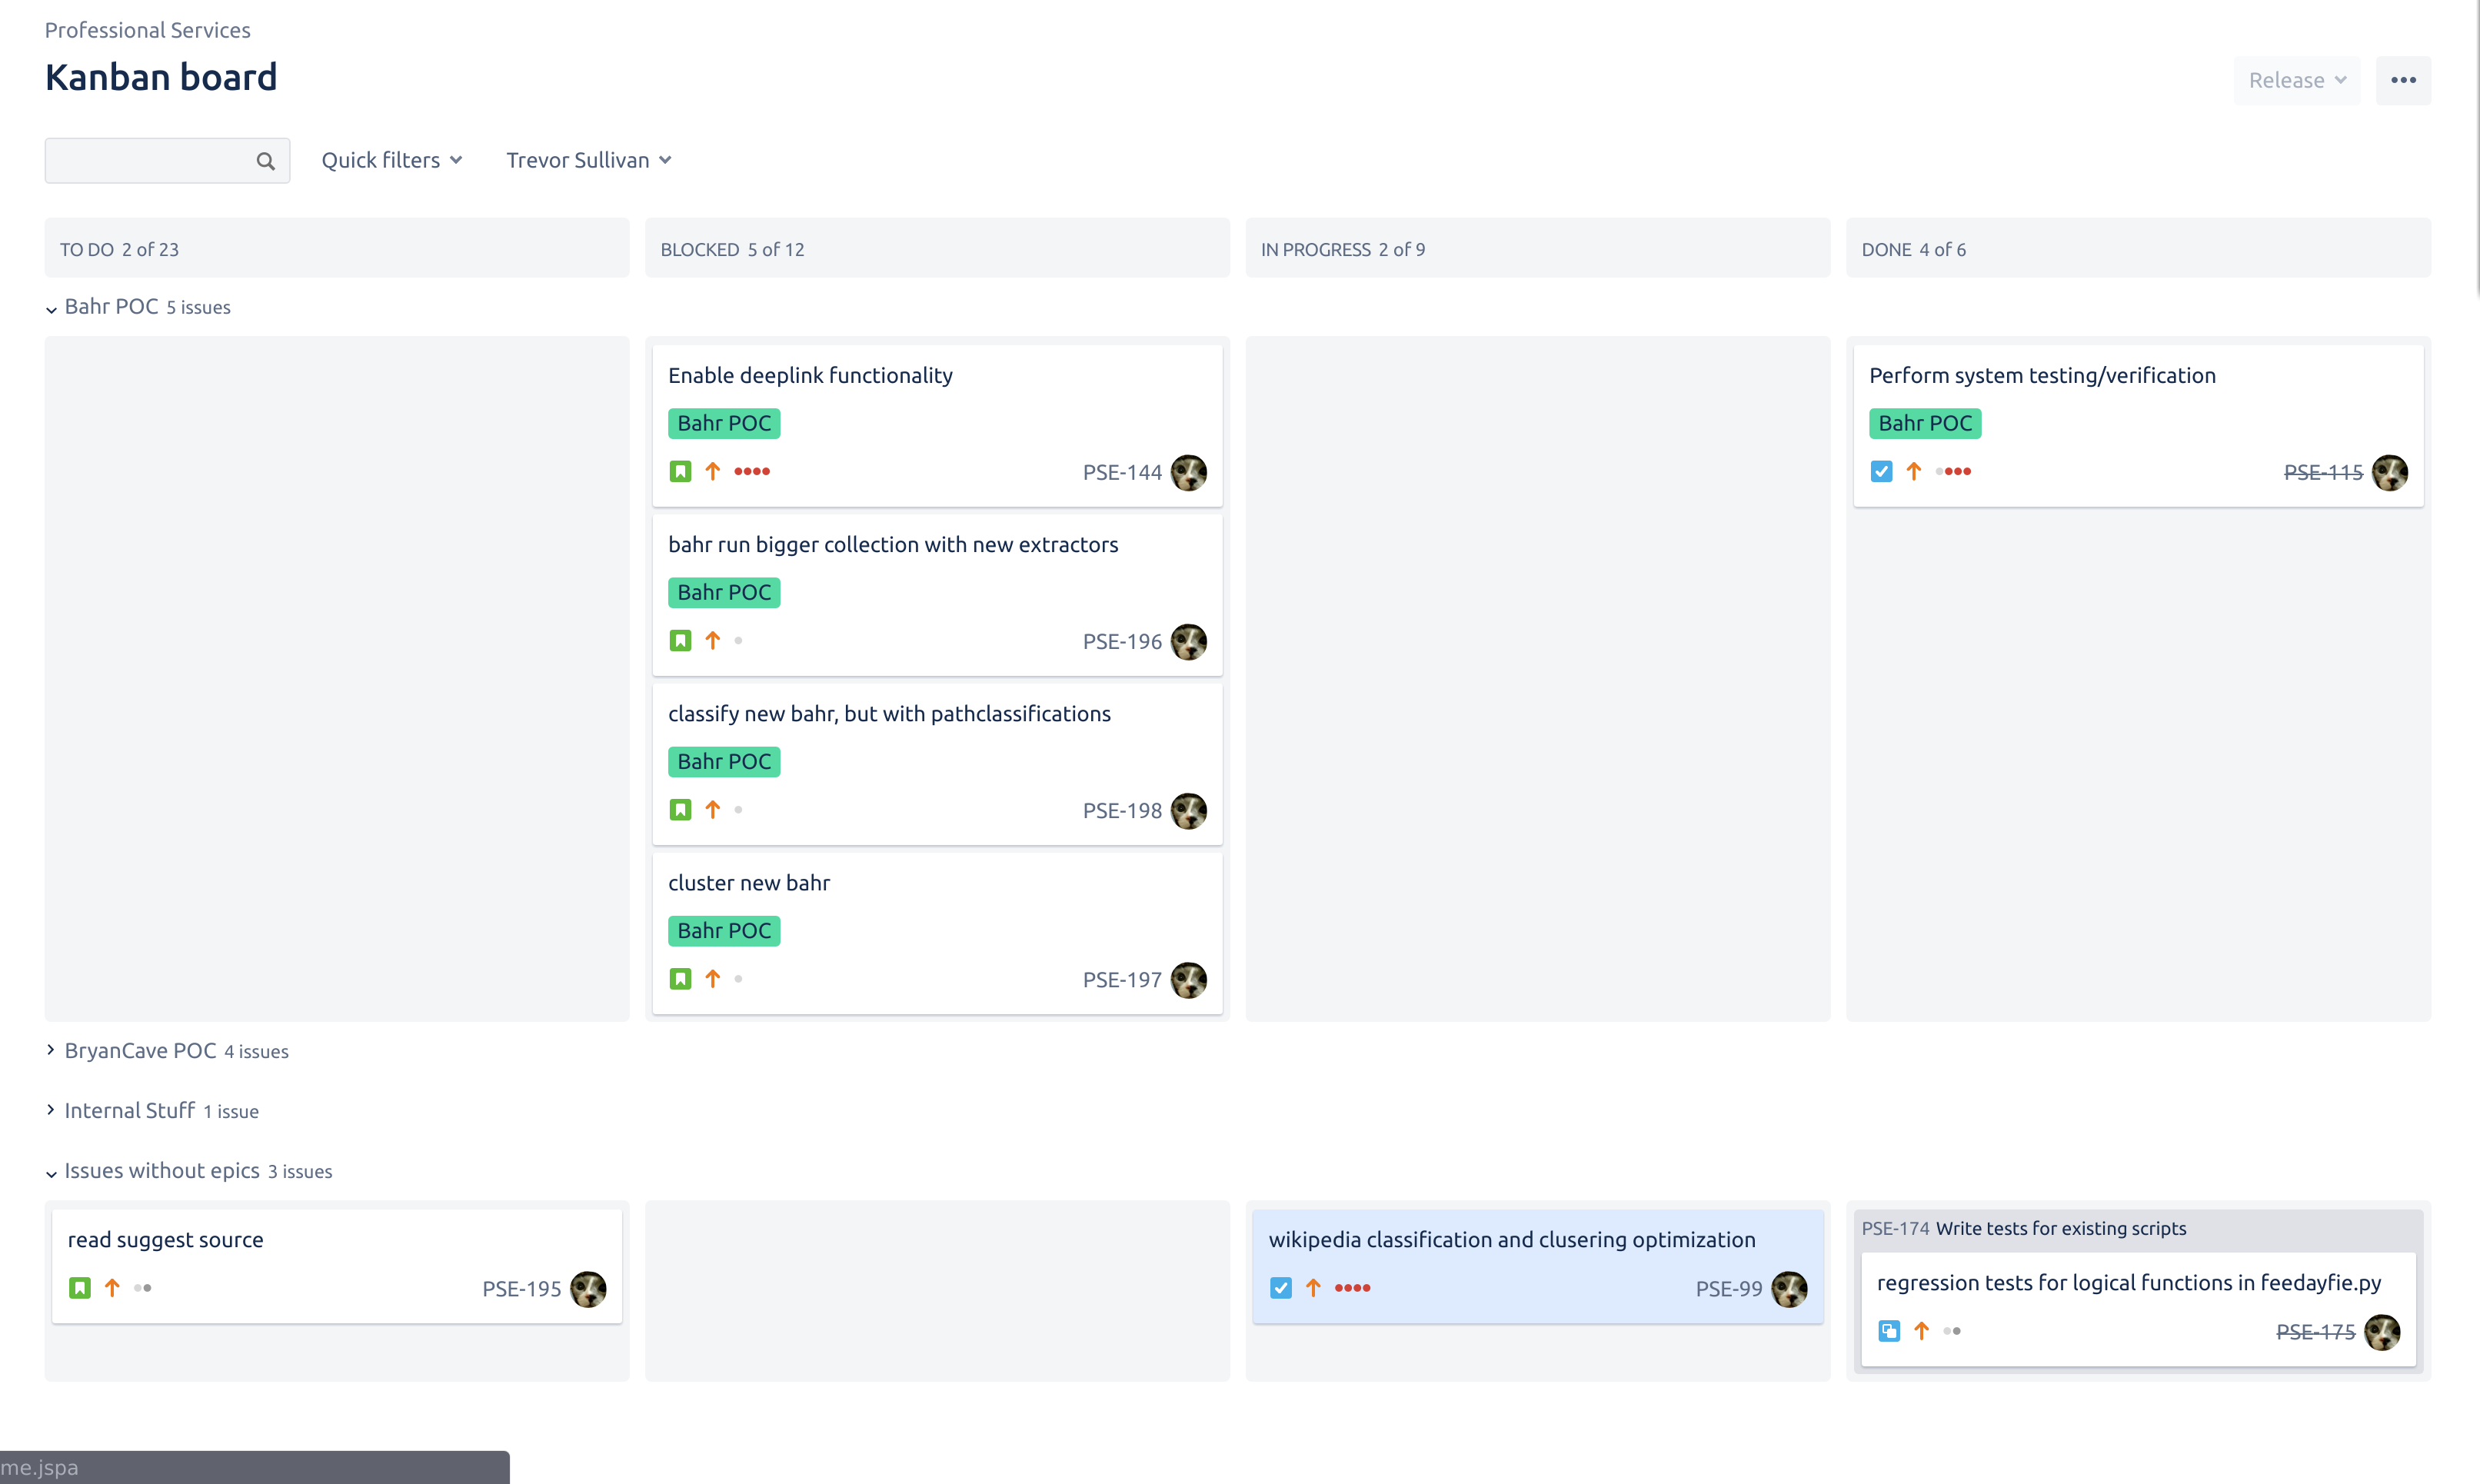
\includegraphics[width=10cm]{figs/pseboard.png}}


\end{frame}

\begin{frame}[c]{Boards}
    \centerline{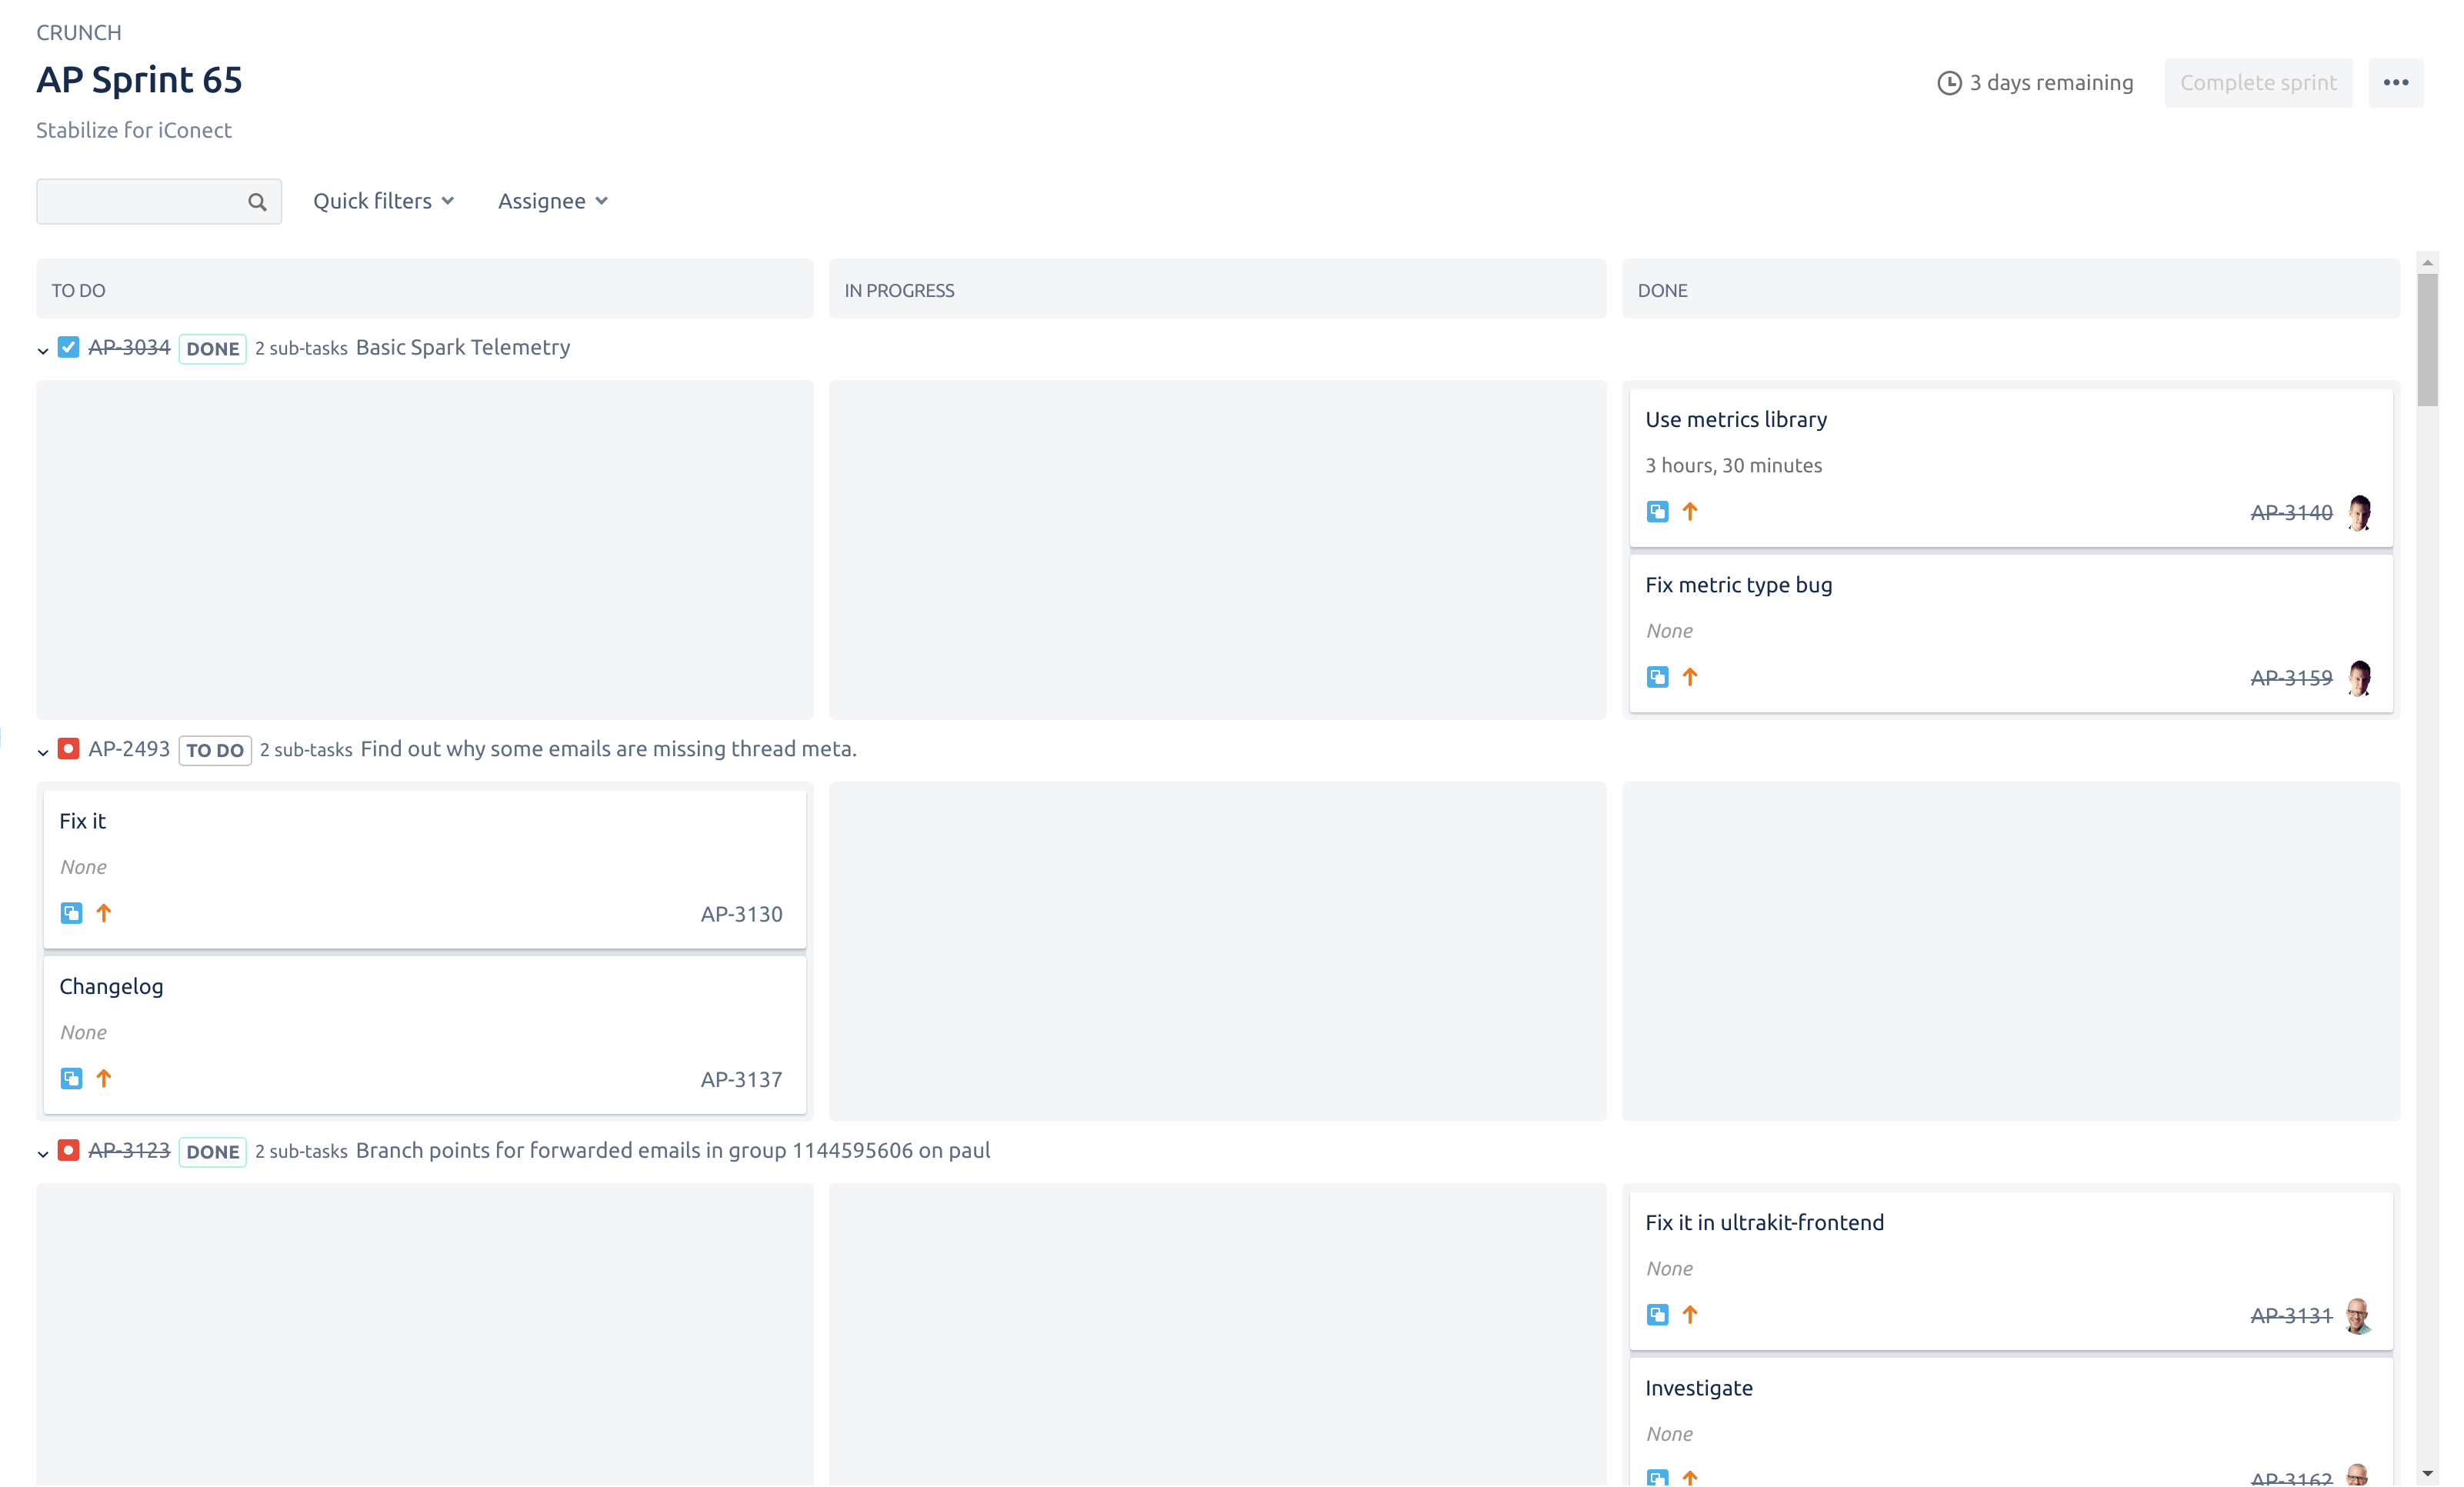
\includegraphics[width=10cm]{figs/apboard.png}}

\end{frame}

\begin{frame}[c]{Do it now: Task Management}
    \begin{itemize}[<+->]
    	\item People tend to overestimate their own ability to remember things
    	\item There is a limited amount of space in your working memory, and to commit something to long term memory, you need to call it back to working memory several times
    	\item This is a waste of brain power. Everything you have to remember distracts you.
    	\item Strive therefore to get things out of your head as soon as possible

    \end{itemize}


\end{frame}

\begin{frame}[c]{Apps: Asana}

\centerline{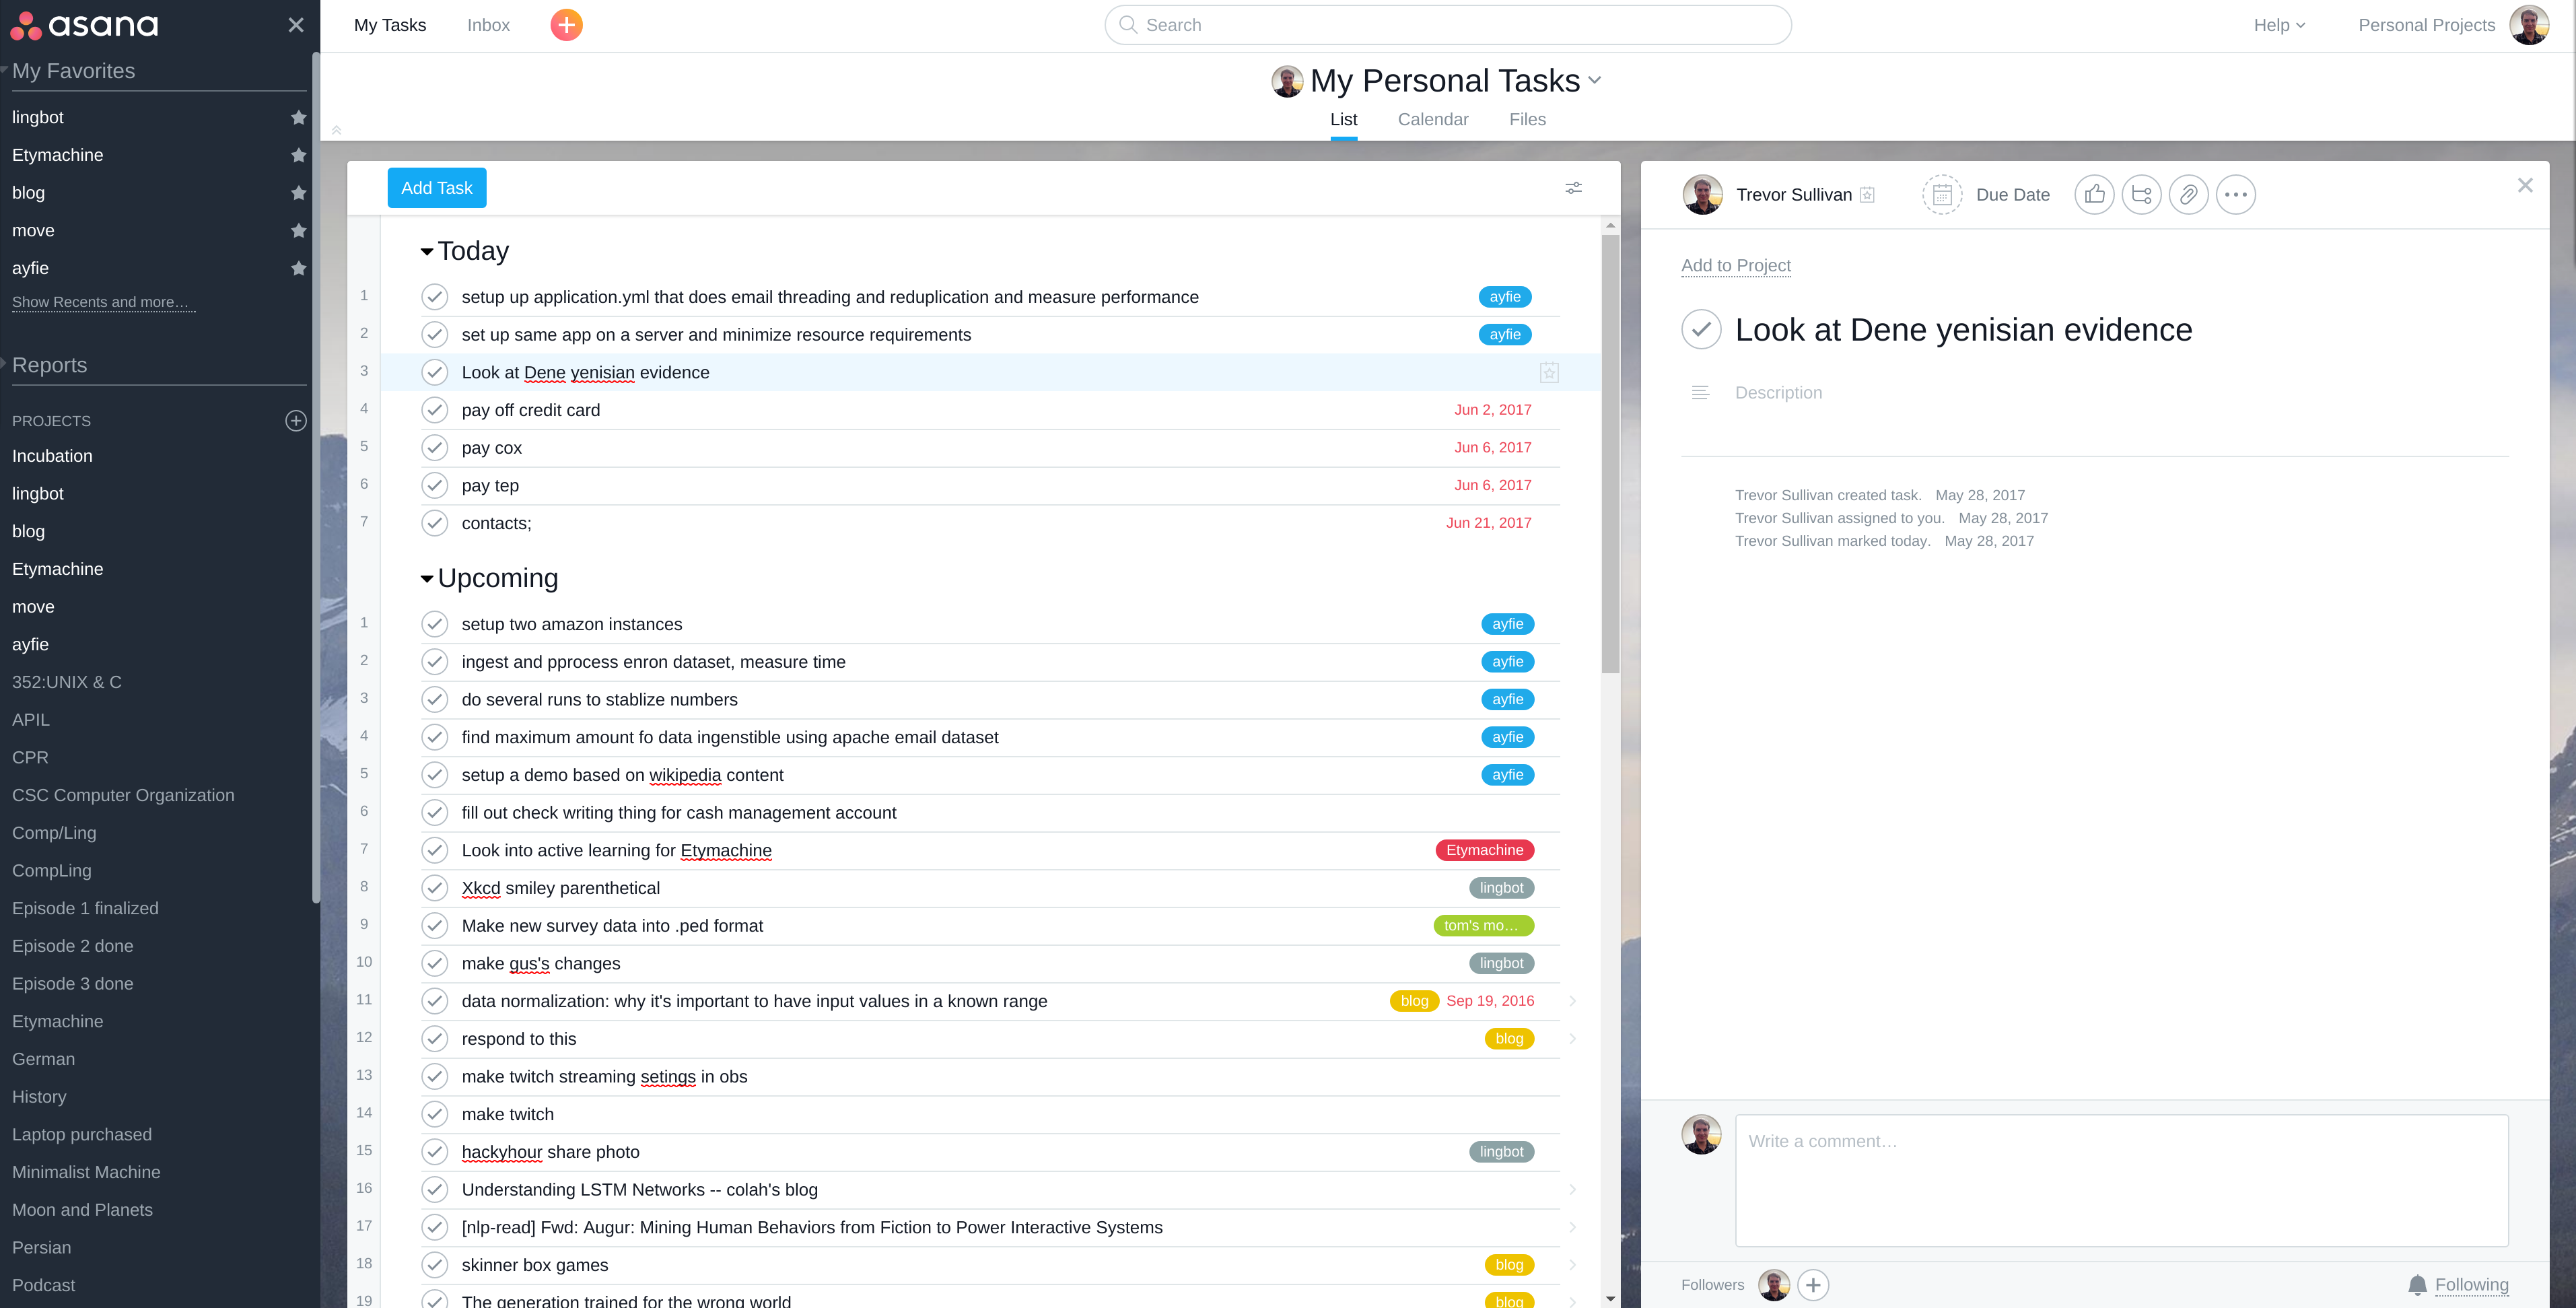
\includegraphics[width=12cm]{figs/asana.png}}

\end{frame}

\begin{frame}[c]{Apps: Todoist}

\centerline{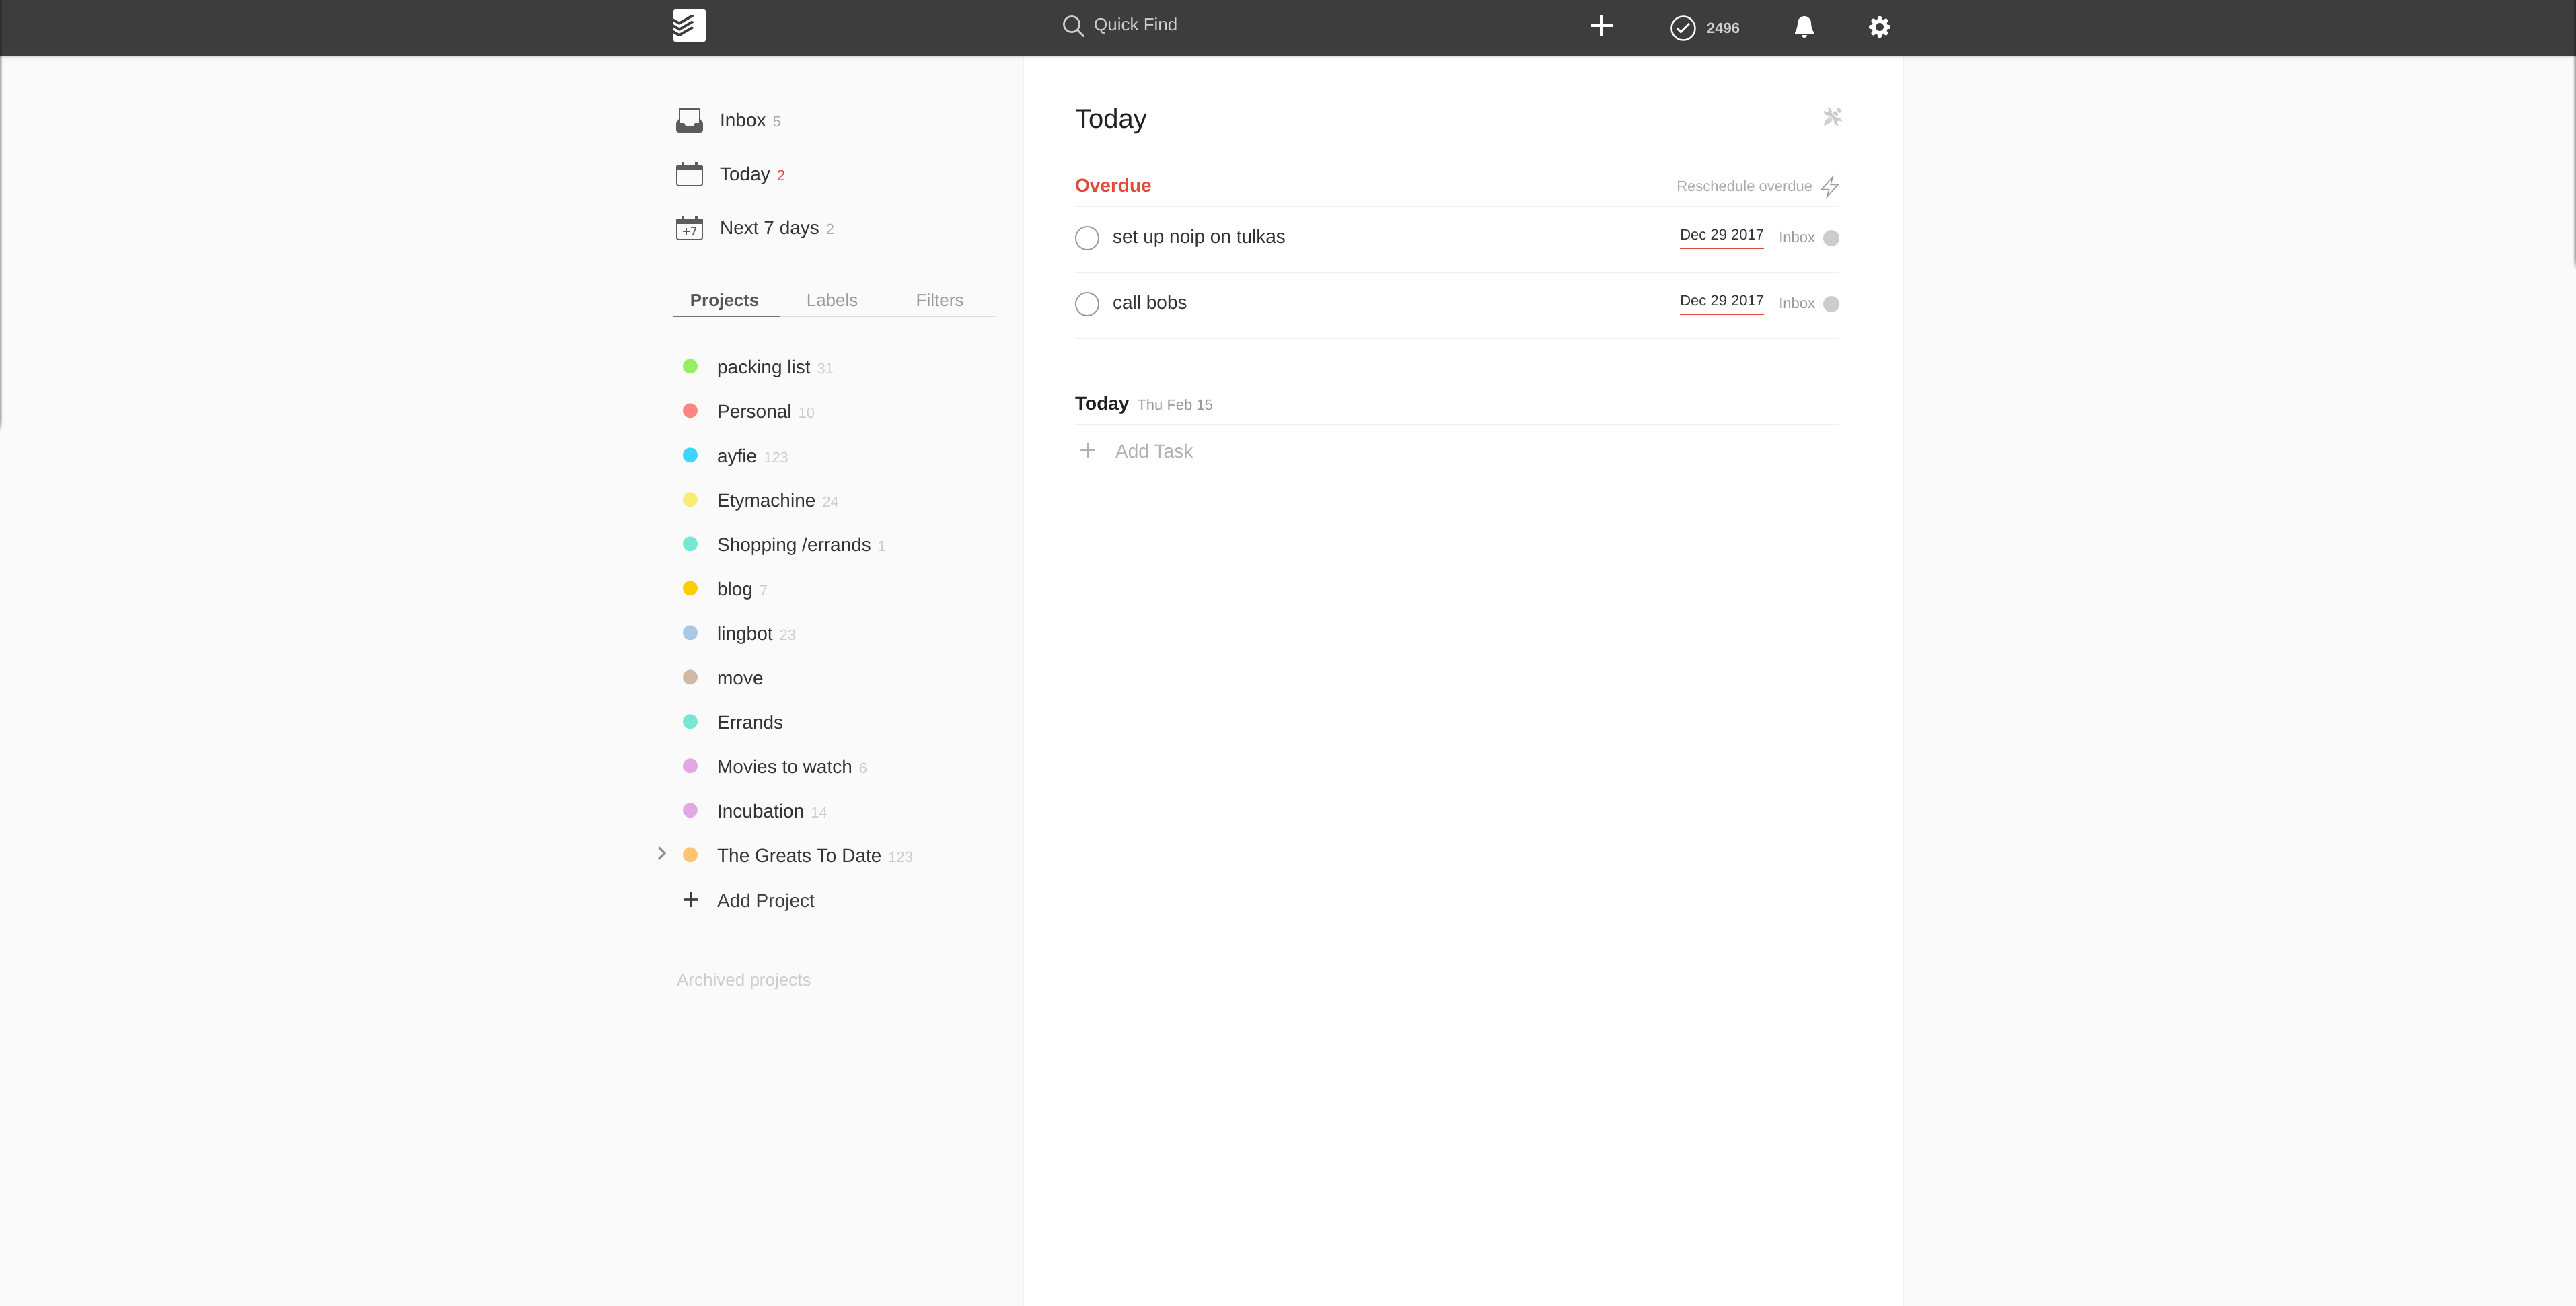
\includegraphics[width=12cm]{figs/todoist.png}}

\end{frame}

\begin{frame}[c]{Apps: HabitRPG}

\centerline{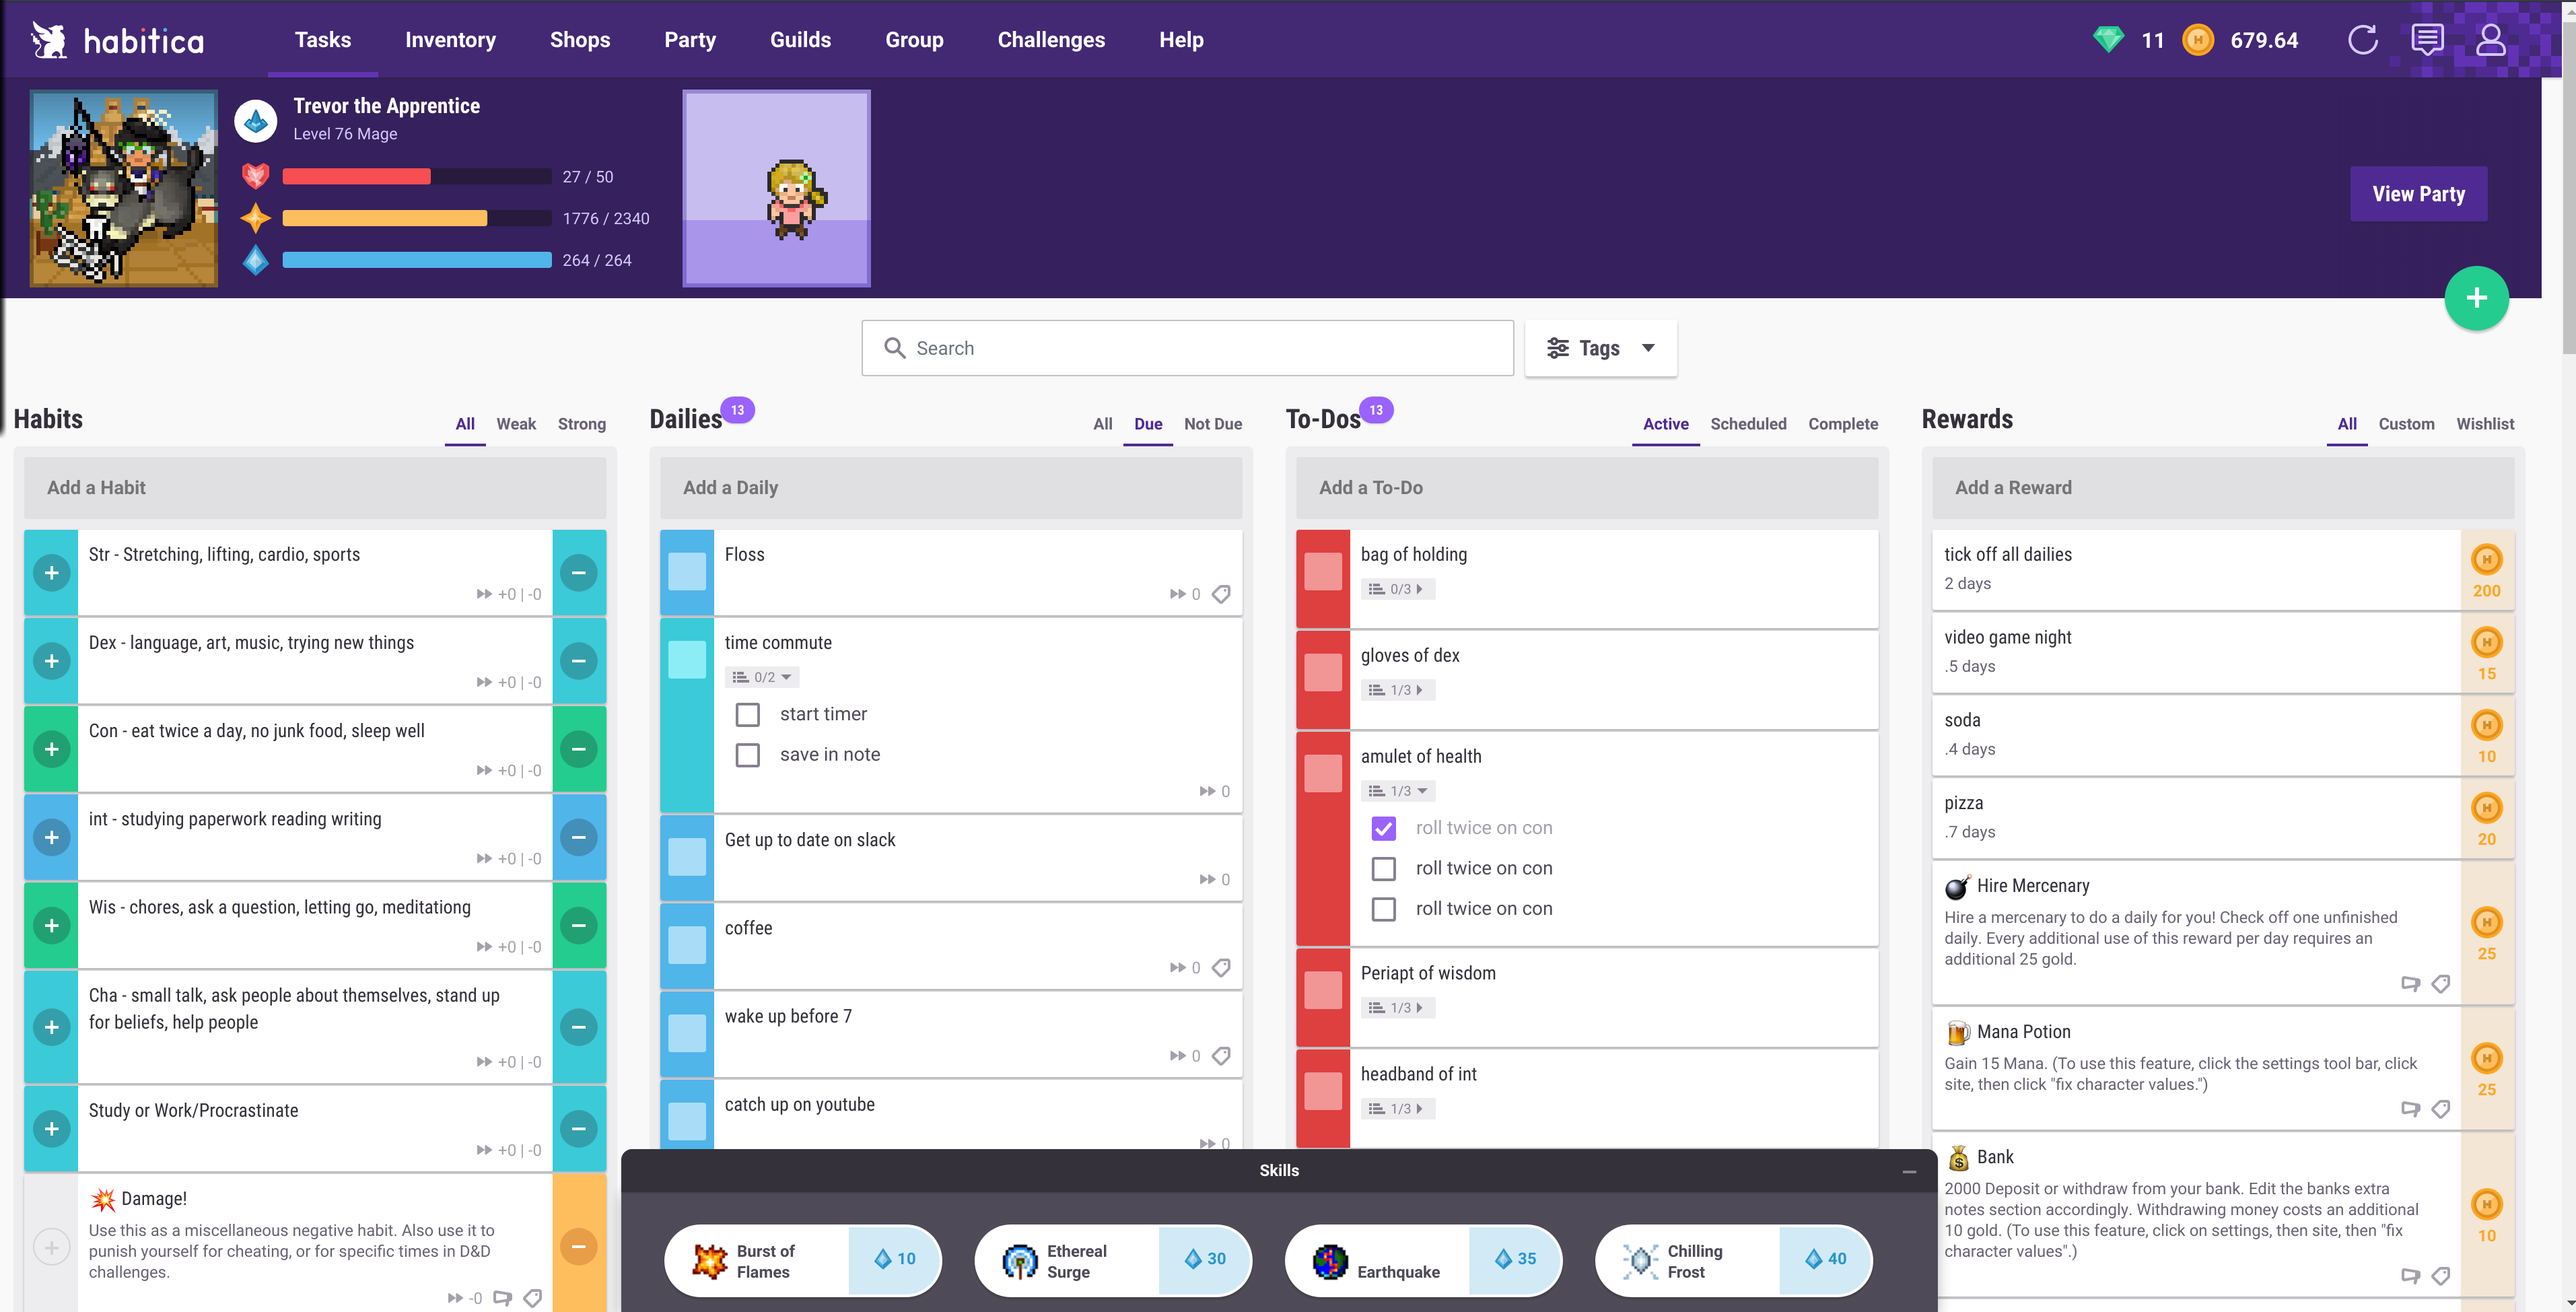
\includegraphics[width=12cm]{figs/habitica.png}}

\end{frame}

\begin{frame}[c]{Apps: Trello}

\centerline{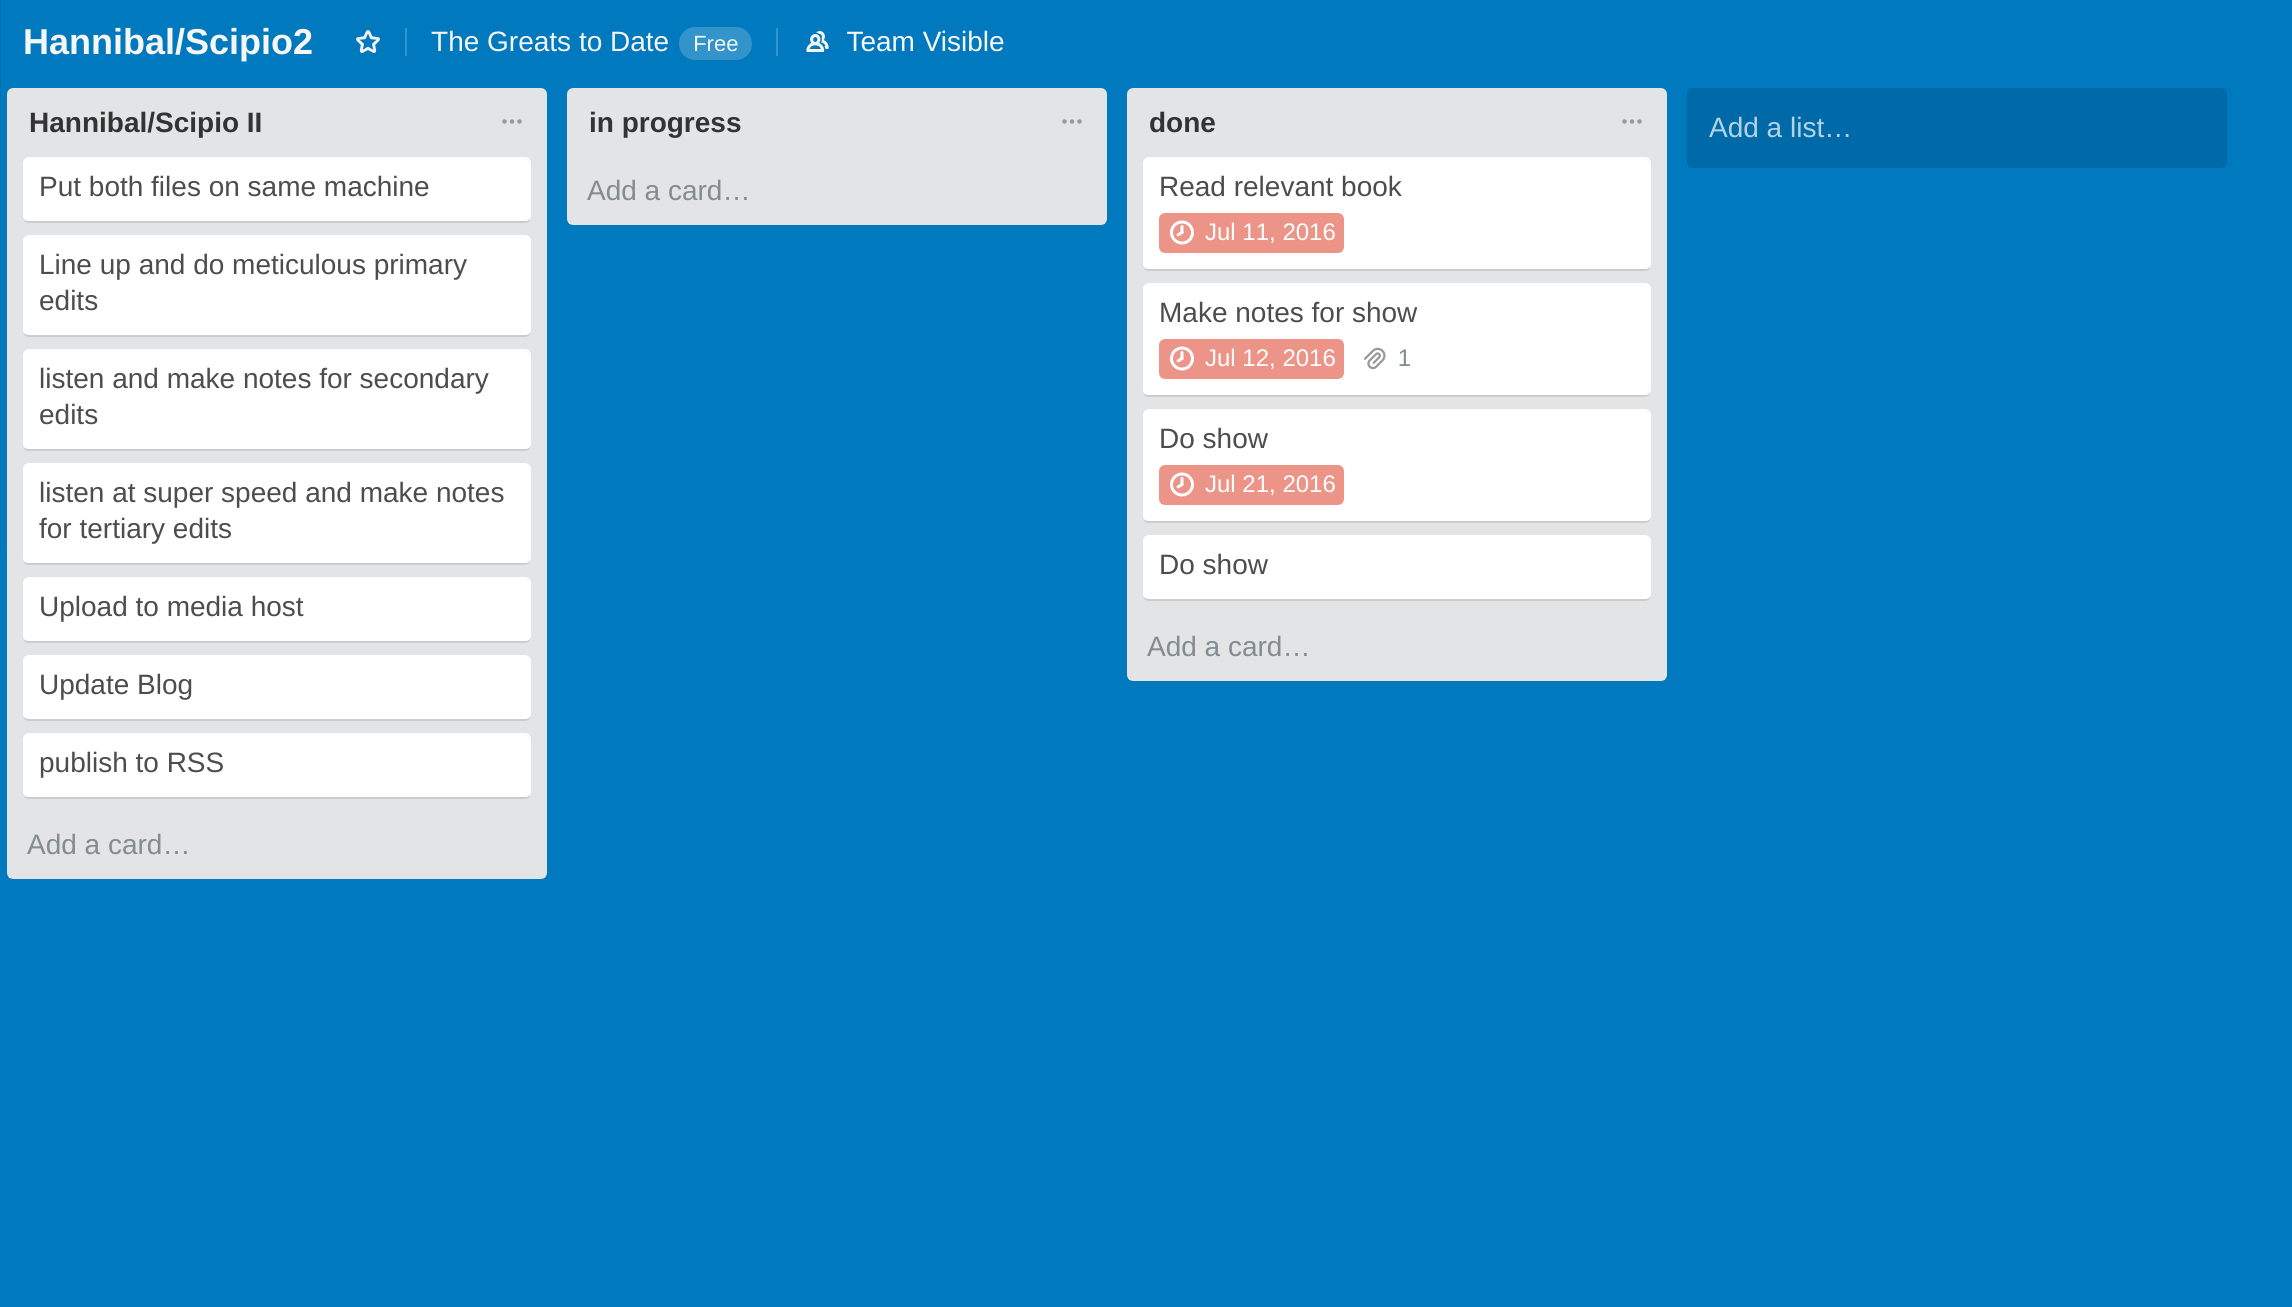
\includegraphics[width=12cm]{figs/trello.png}}

\end{frame}

\begin{frame}[c]{Apps: todo.txt}

\centerline{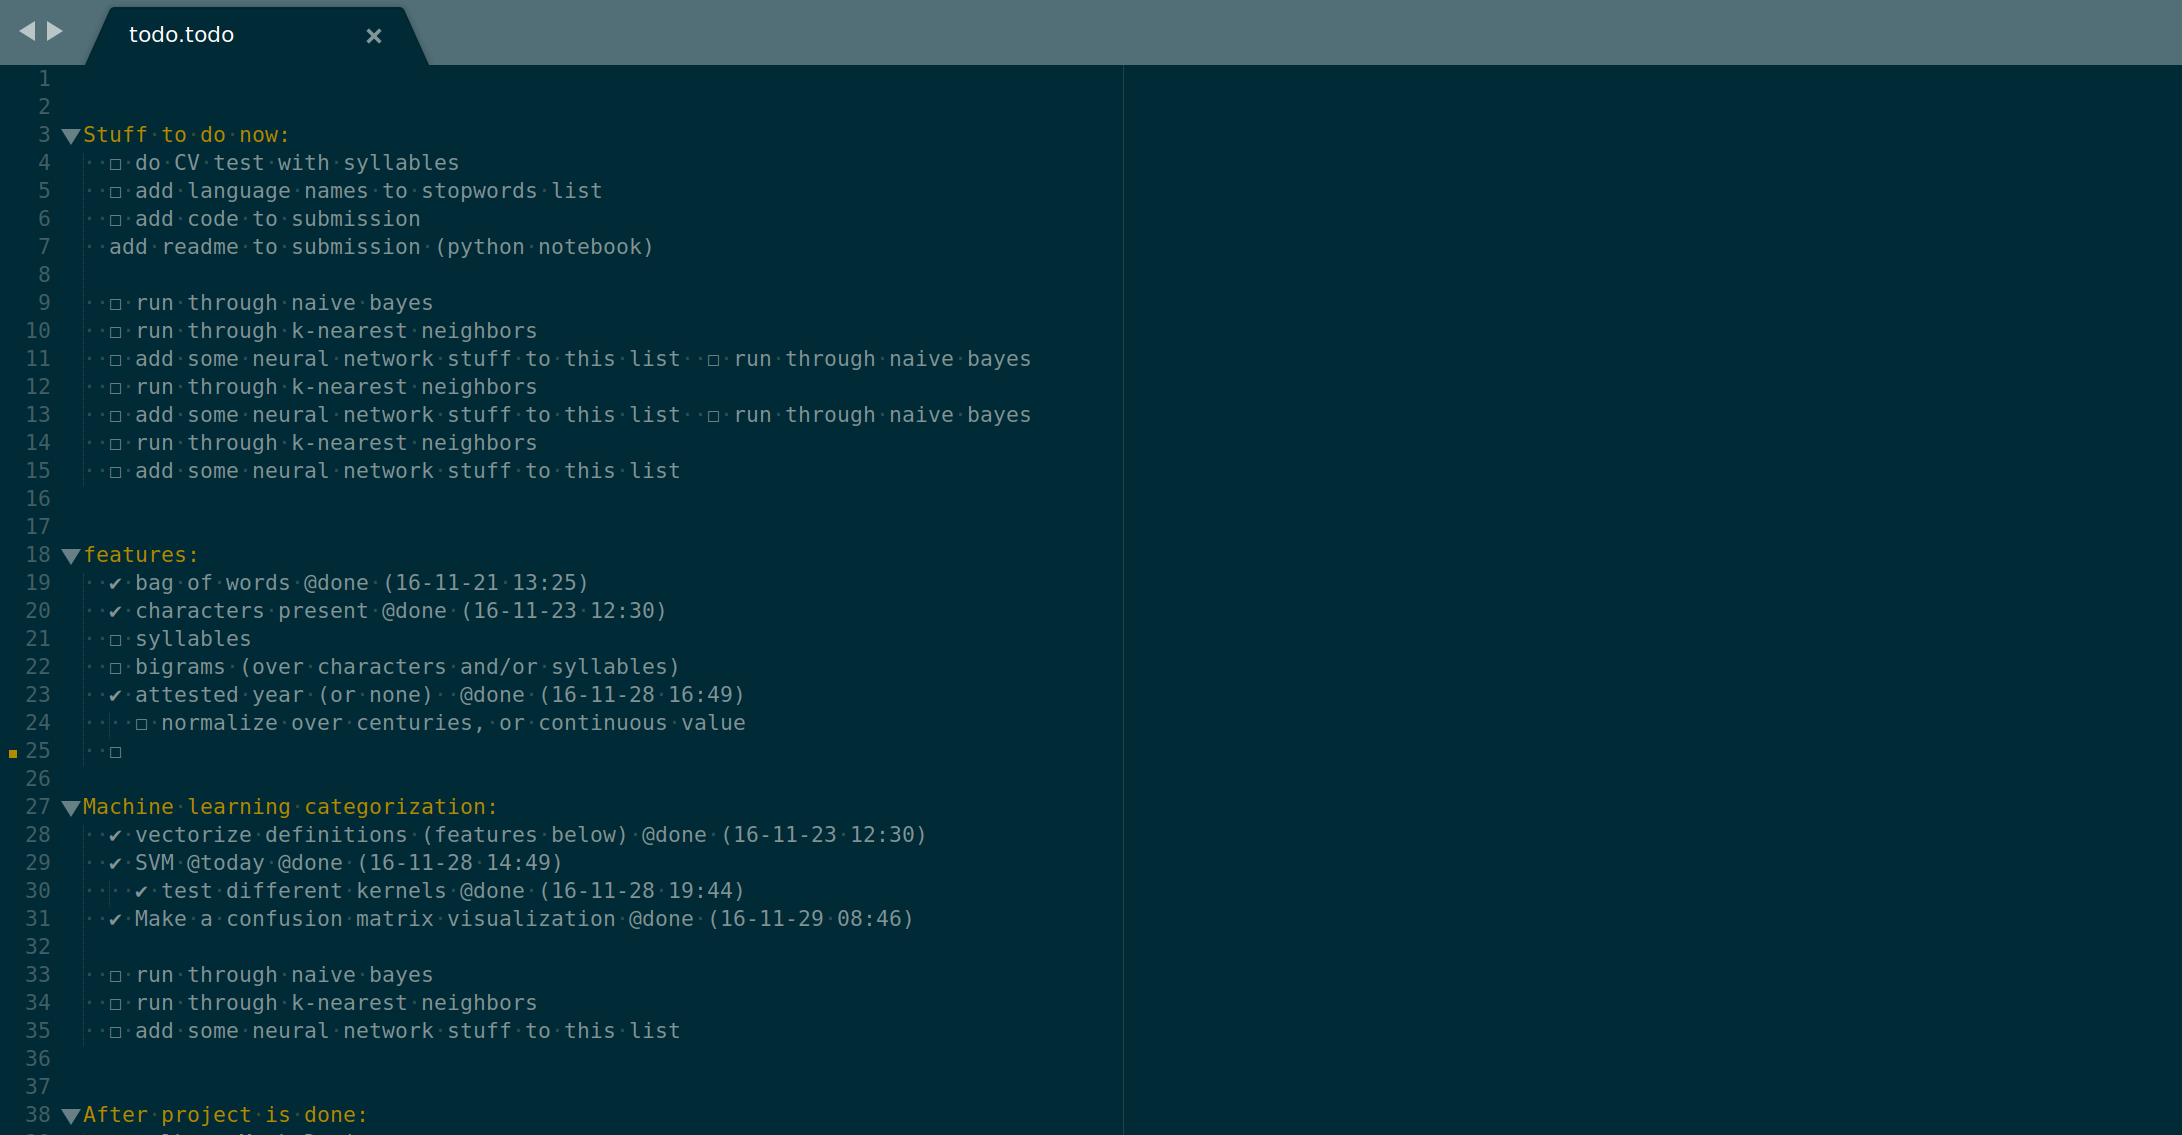
\includegraphics[width=12cm]{figs/todotxt.png}}

\end{frame}

\begin{frame}[c]{Apps: Bulletjournal}

\centerline{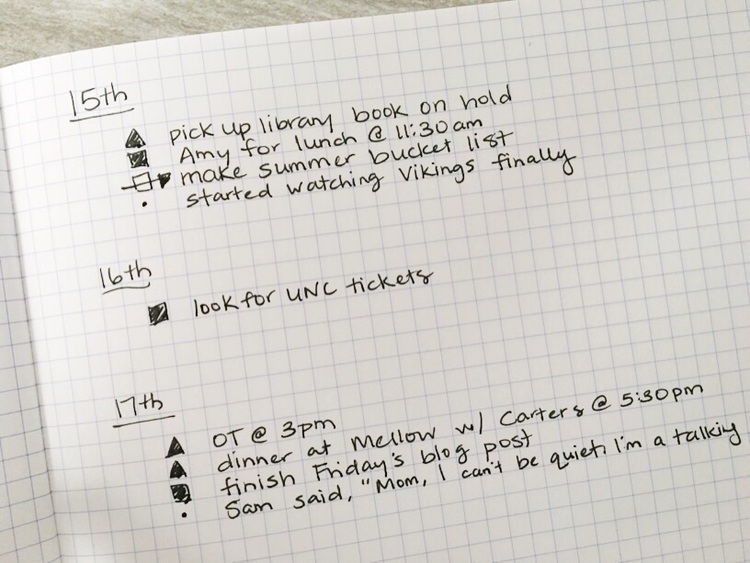
\includegraphics[width=12cm]{figs/bulletjournal.jpeg}}

\end{frame}

\begin{frame}[c]\frametitle{Advanced: Time tracking}

Not essential, but if you already have a good system for keeping track of your tasks.

\centerline{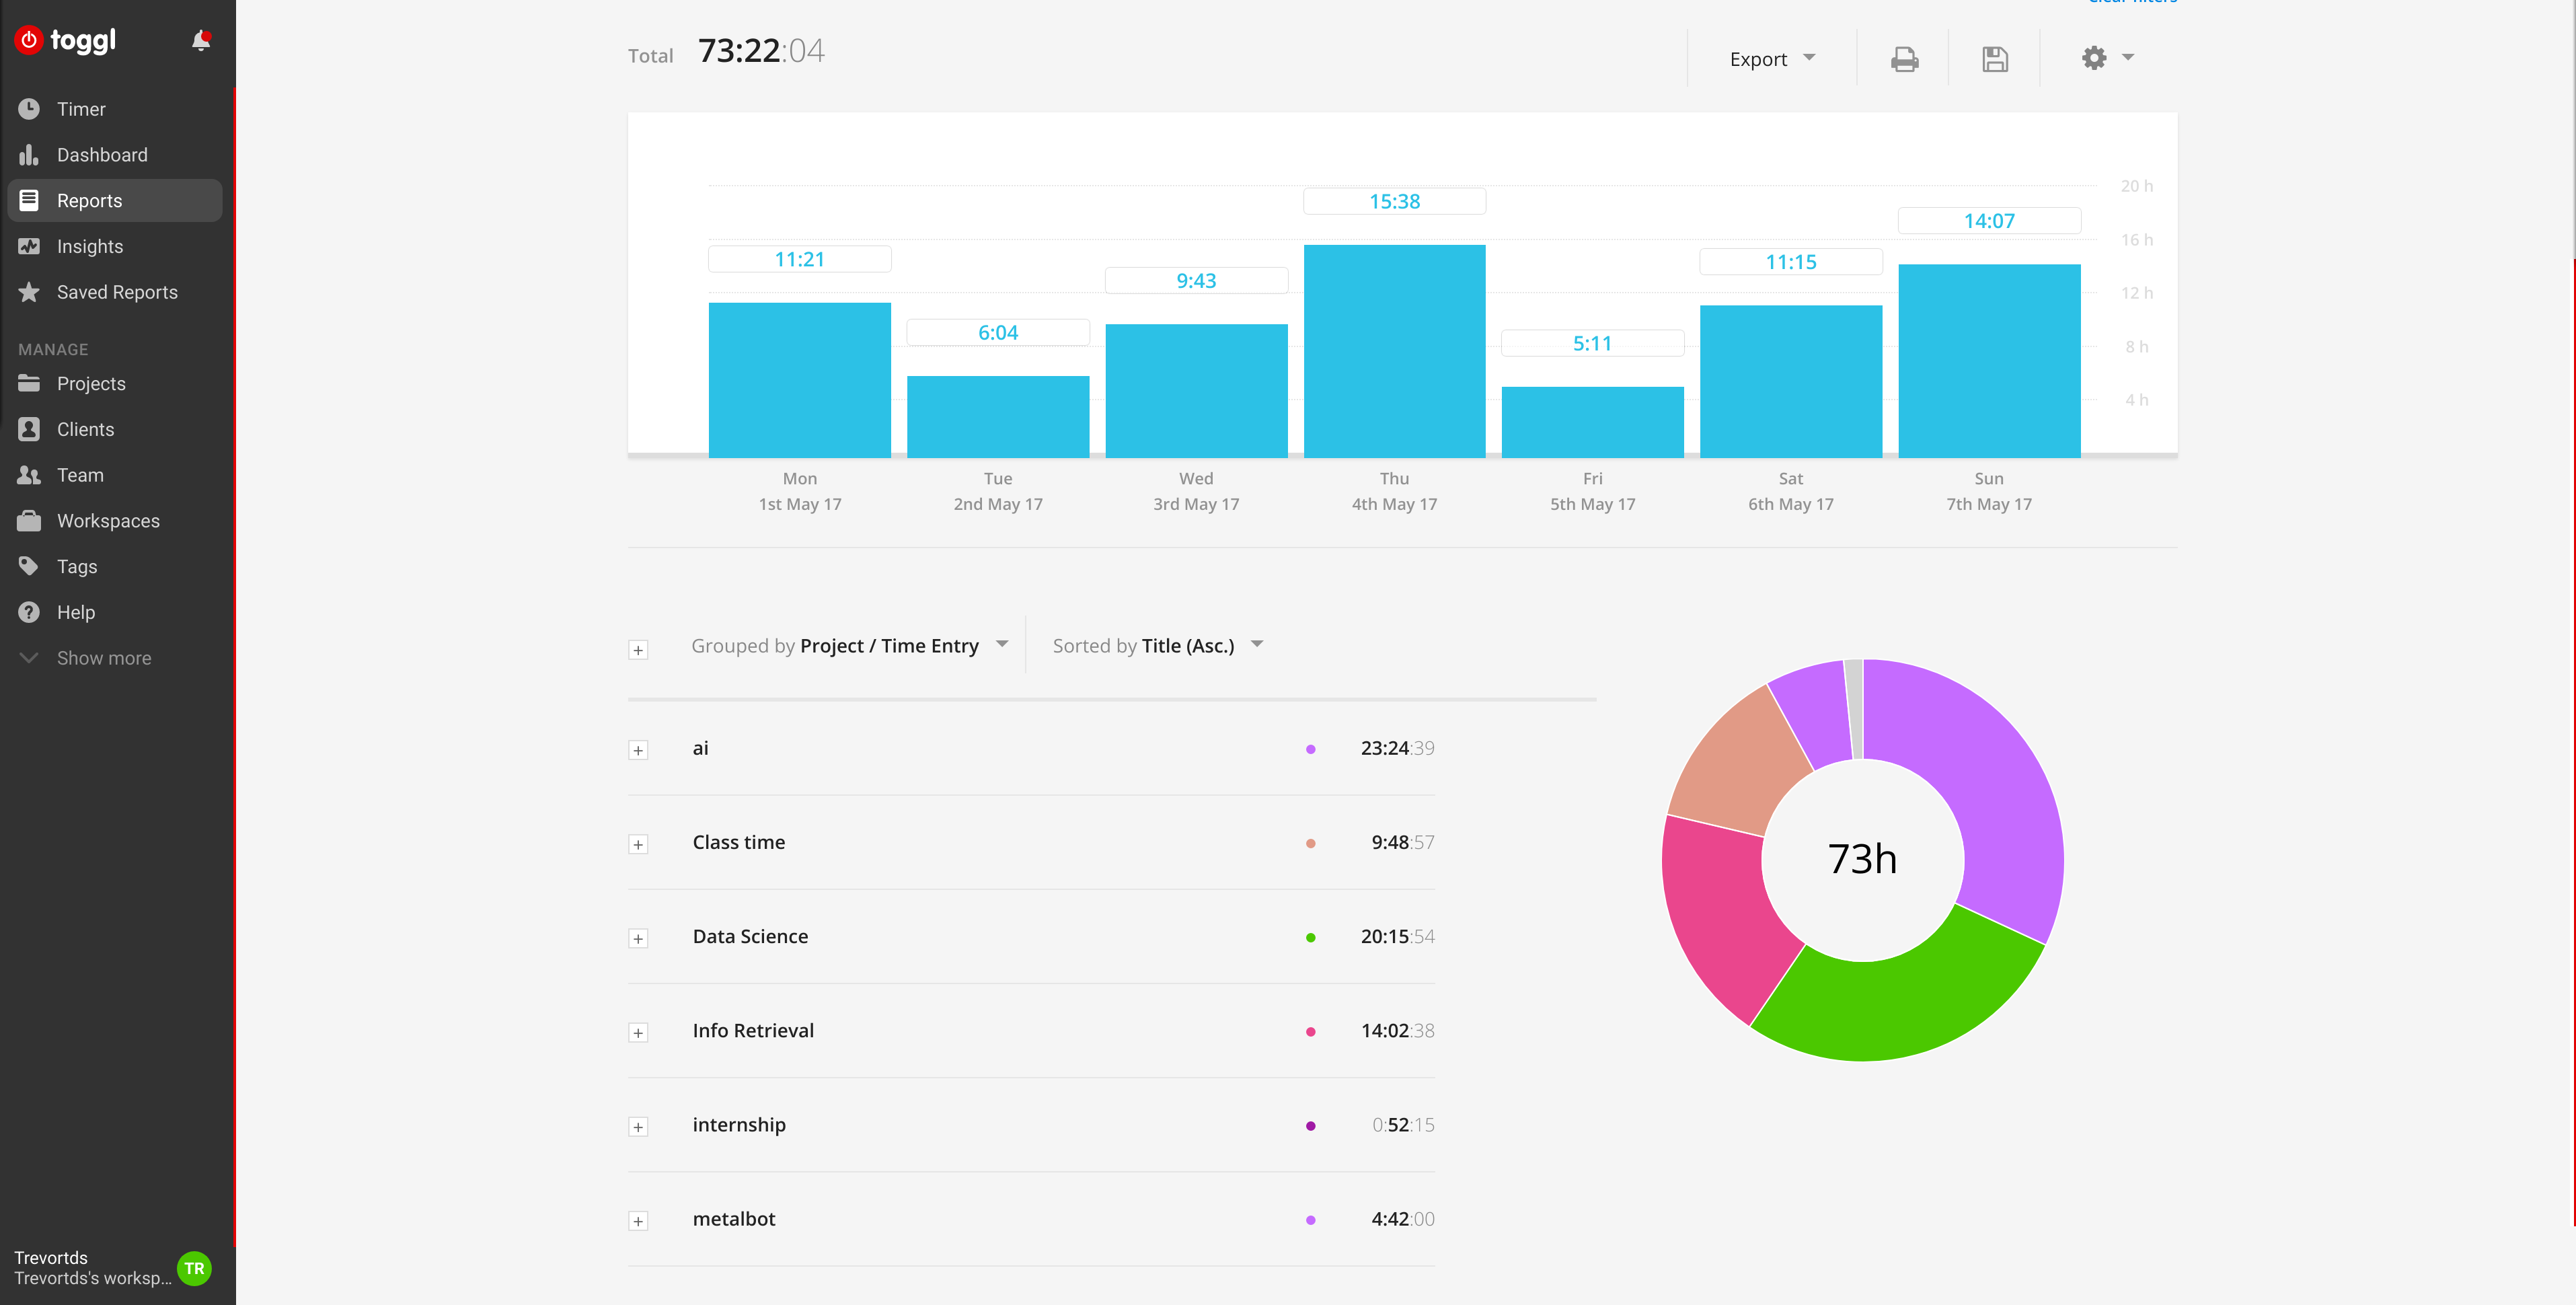
\includegraphics[width=10cm]{figs/toggl.png}}

\end{frame}

\begin{frame}[c]\frametitle{Super-Advanced: Automation}

Many of the aforementioned apps have APIs that can be manipulated manually, or through Zapier

\centerline{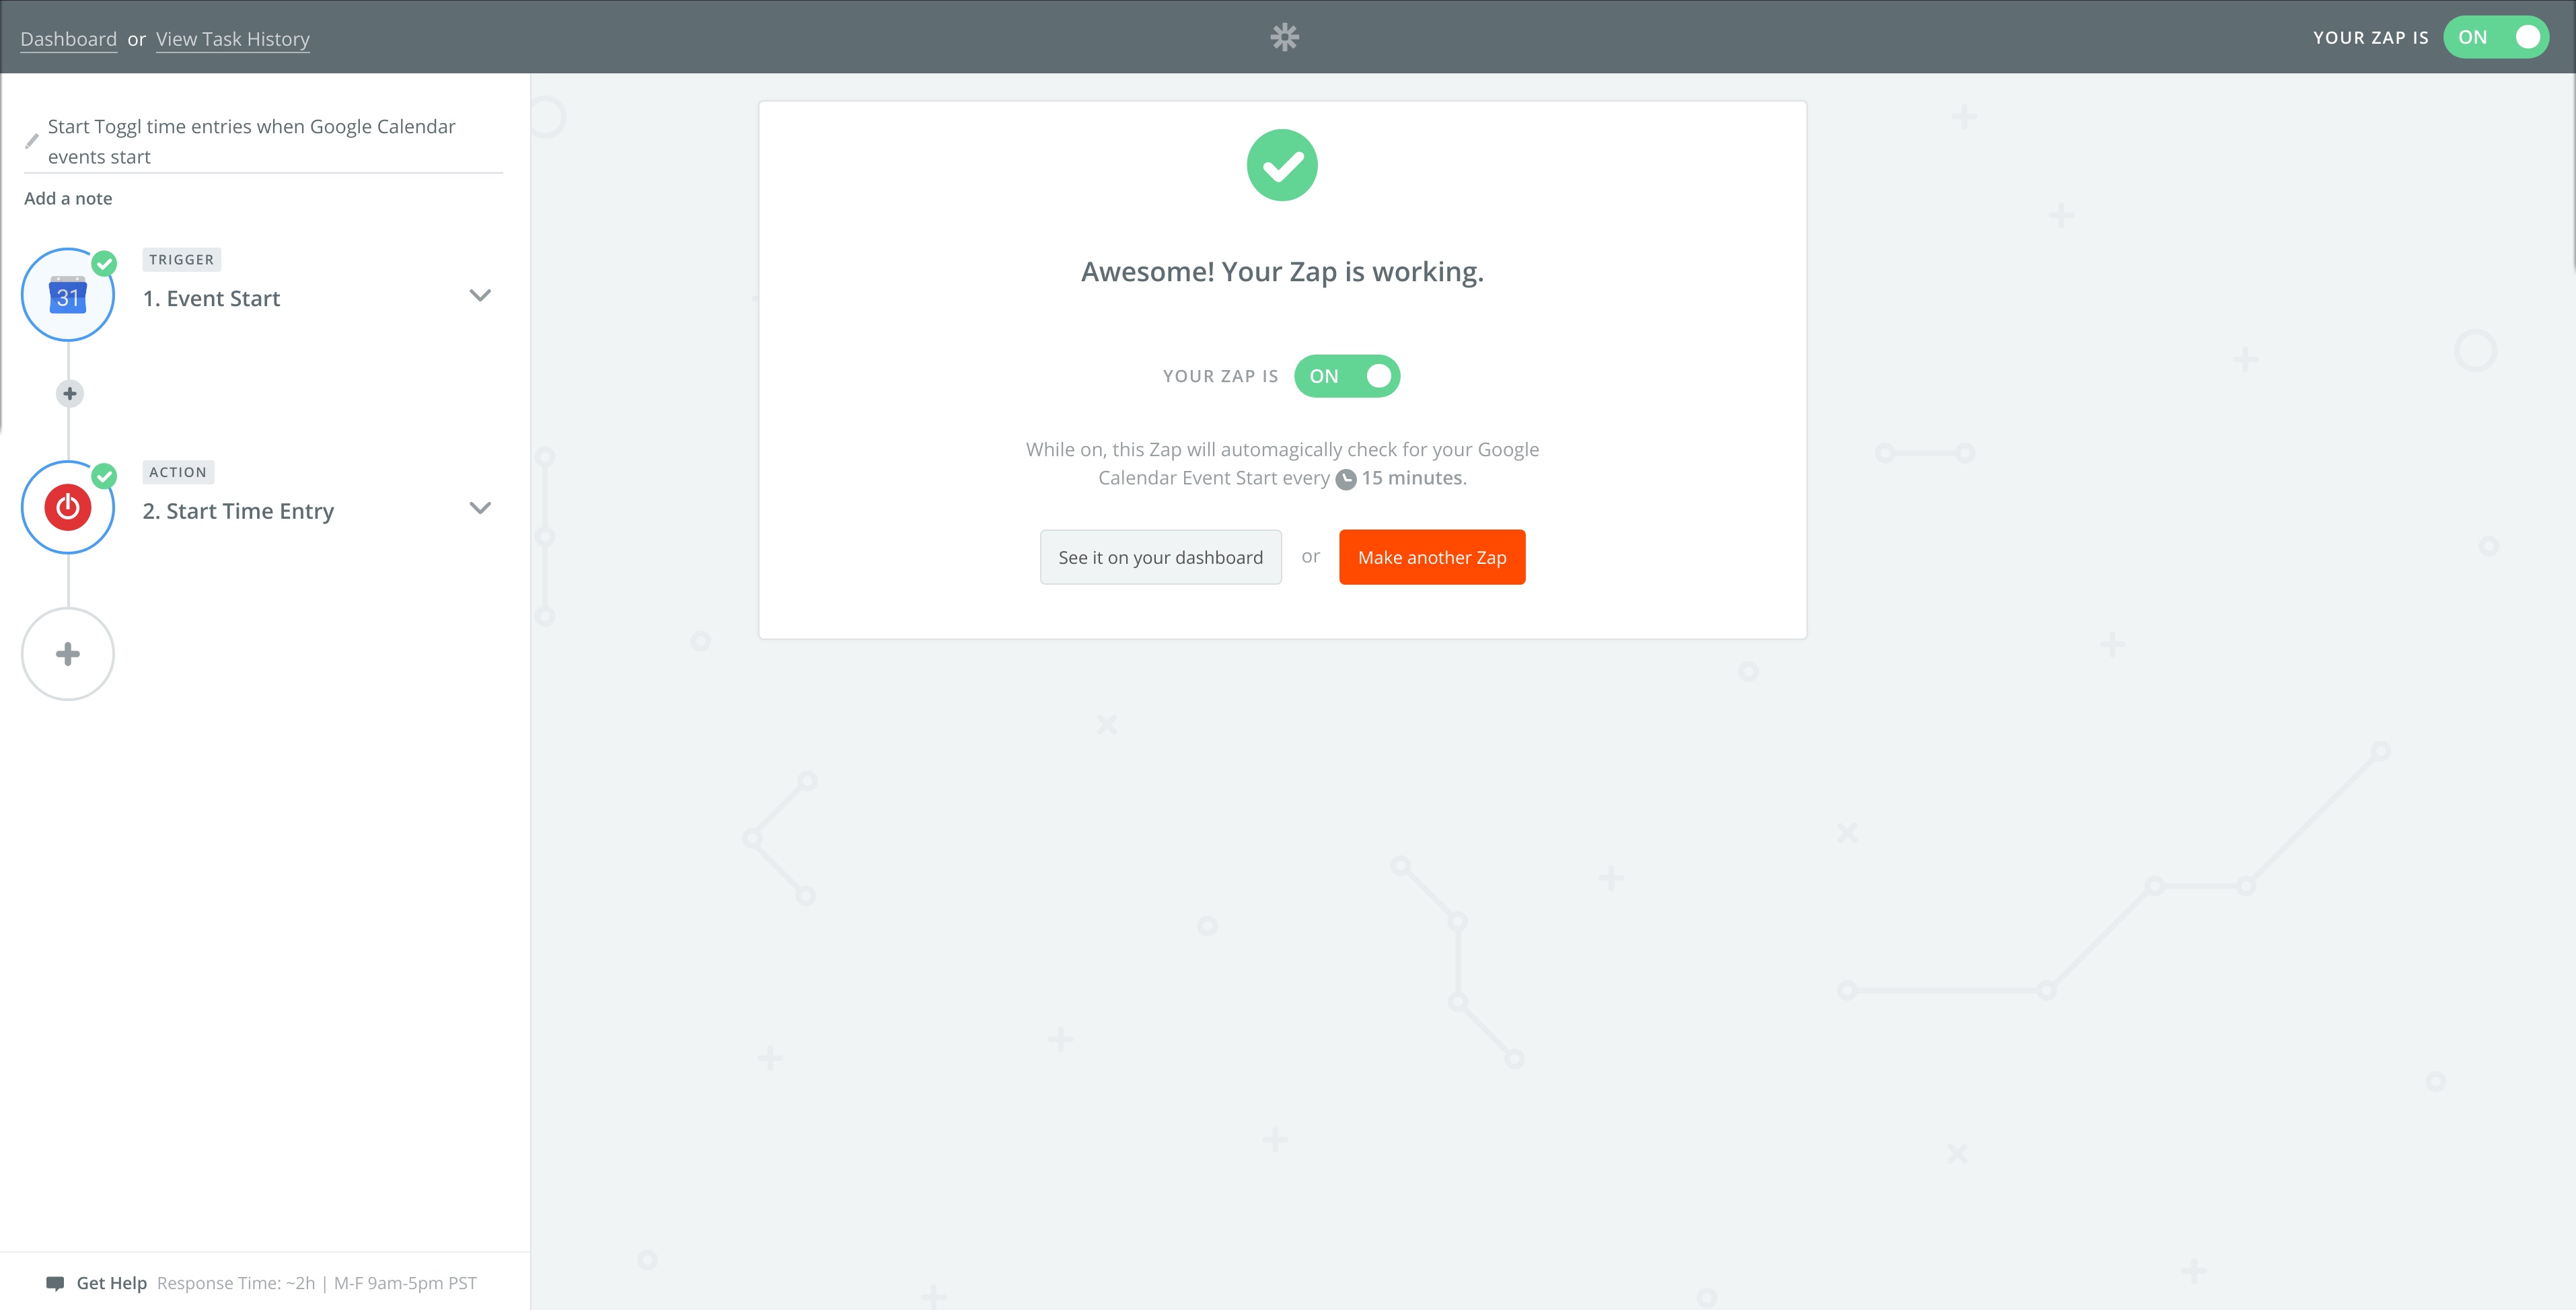
\includegraphics[width=10cm]{zapier.png}}

\end{frame}













\section{System Administration | The Command Line}


\begin{frame}[c]
	\frametitle{Be aware of: Finer points of sysadmin}
	\pause
	When you're working on a server. you will need to learn some particular skills and methods to manage things

	\begin{description}[<+->]
		\item[Managing volumes] \texttt{df -h}, \texttt{fdisk}, \texttt{mkfs}
		\item[ssh tunnels and UDP] \texttt{ssh -L 18080:127.0.0.1:18085 -R 18086:127.0.0.1:18086 user@server}
		\item[web access control]  \texttt{nginx}
	\end{description}
\end{frame}


\begin{frame}[c]
	\frametitle{Do it now: The Command Line}
	\begin{itemize}[<+->]
		\item Navigating a *nix filesystem
		\item text editor (vim, emacs, nano)
		\item tmux or screen

		They may seem dumb at first, but you will soon find you can't live without it

		Like browsing without tabs
	\end{itemize}
\end{frame}

\begin{frame}[c]
	\frametitle{tmux}

	\centerline{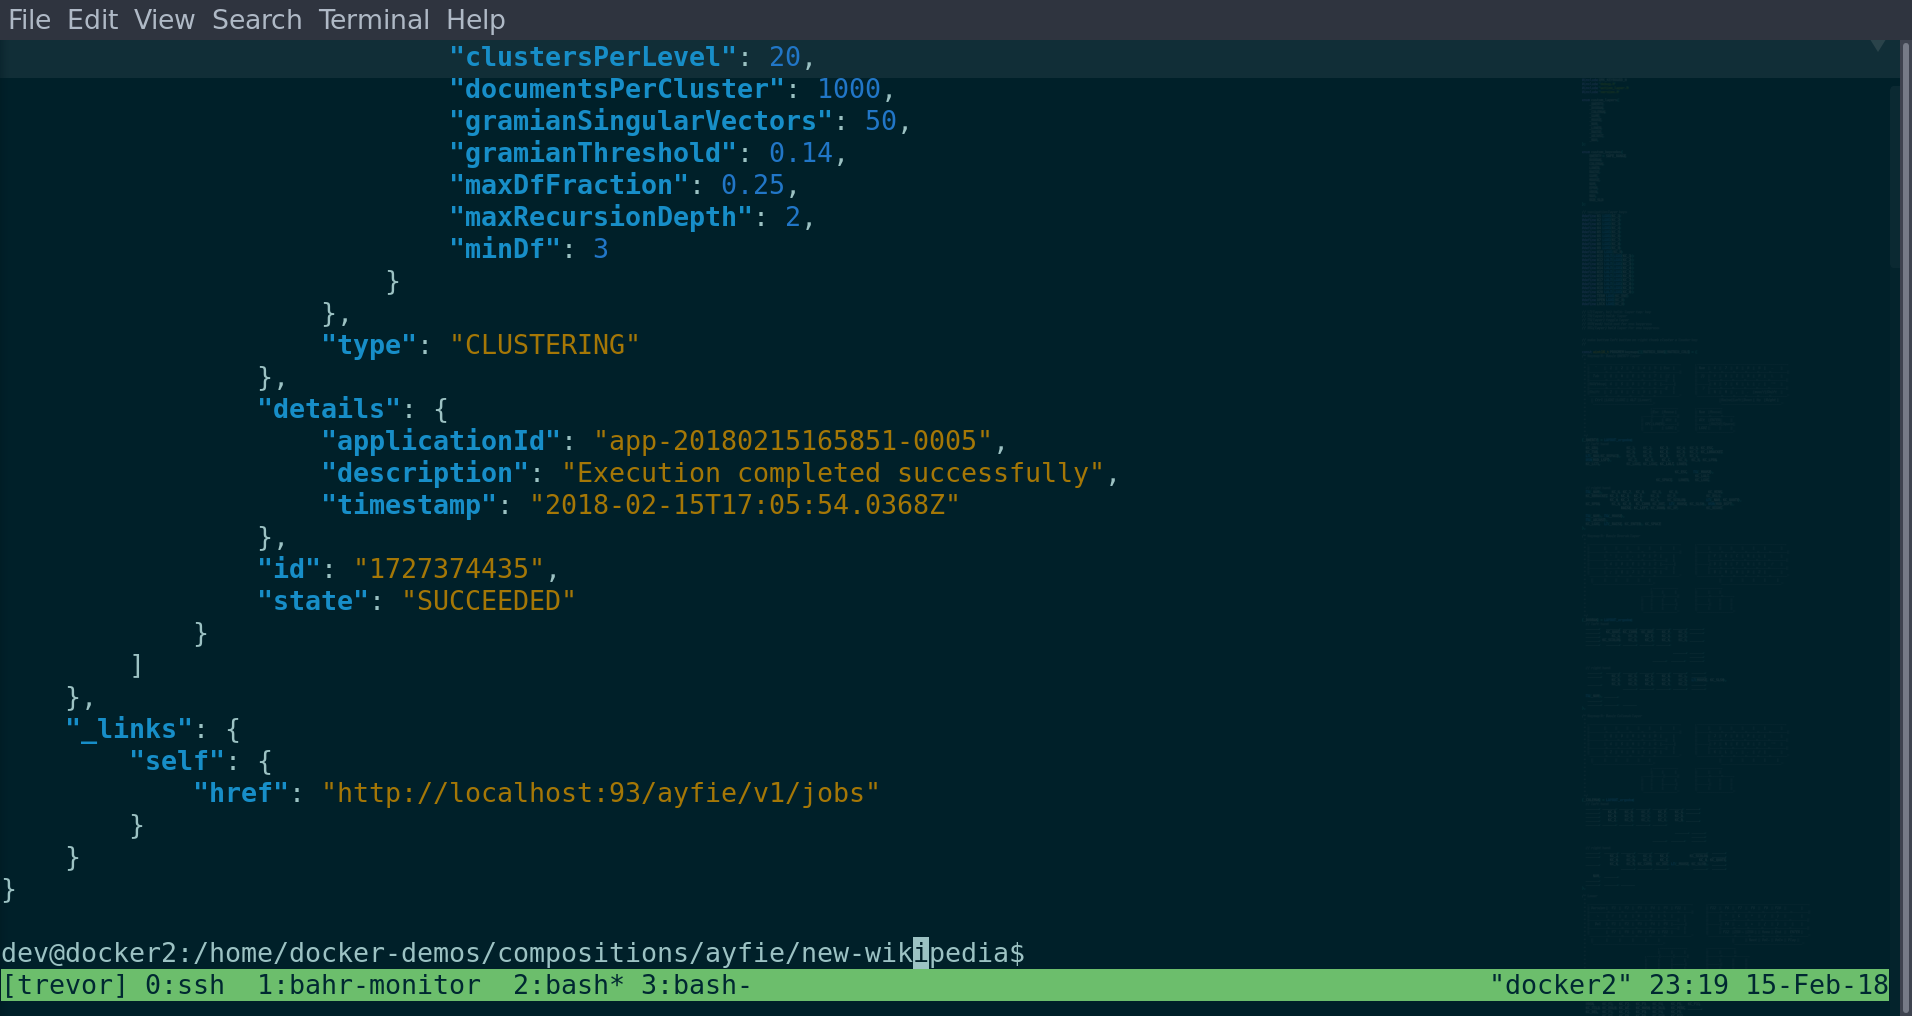
\includegraphics[width=12cm]{tmux.png}}
\end{frame}









\begin{frame}[standout]
  That's all!
\end{frame}





\end{document}
